\documentclass{acmsiggraph}               % final
%\documentclass[review]{acmsiggraph}      % review
%\documentclass[widereview]{acmsiggraph}  % wide-spaced review
%\documentclass[preprint]{acmsiggraph}    % preprint

%% Uncomment one of the four lines above depending on where your paper is
%% in the conference process. ``review'' and ``widereview'' are for review
%% submission, ``preprint'' is for pre-publication, and ``final'' is for
%% the version to be printed.

%% These two line bring in essential packages: ``mathptmx'' for Type 1 
%% typefaces, and ``graphicx'' for inclusion of EPS figures.

\usepackage{mathptmx}
\usepackage{graphicx}

%% use this for zero \parindent and non-zero \parskip, intelligently.

\usepackage{parskip}

%% If you are submitting a paper to the annual conference, please replace 
%% the value ``0'' below with your OnlineID. If you are not submitting this
%% paper to the annual conference, you may safely leave it at ``0'' -- it 
%% will not be included in the output.

\onlineid{0}

%% need to document this!

\acmformat{print}

%% Paper title.

\title{State of the Art Report - Crowd Simulation}

%% Author and Affiliation (single author).

%%\author{Roy G. Biv\thanks{e-mail: roy.g.biv@aol.com}\\Allied Widgets Research}

%% Author and Affiliation (multiple authors).


\author{Manuel Eiweck\thanks{e-mail: e1633012@student.tuwien.ac.at}\\ Student of Technical University Vienna}

%% Keywords that describe your work.

\keywords{crowd simulation, state of the art report}

%%%%%% START OF THE PAPER %%%%%%

\begin{document}

\teaser{
 \includegraphics[width=\textwidth]{images/bannerImg.png}
 \caption{Example crowd simulations. Left: collision avoidance model \protect\cite{ondrej_synthetic-vision_2010}, middle-left: commercial application MassMotion \protect\cite{mediaworks_pedestrian_2020}, middle-right: crowd behaviour model \protect\cite{pelechano_controlling_2007}, right: bird flock animation, one of the first papers on the crowd simulation field \protect\cite{reynolds_flocks_1987}}
 \label{fig:teaser}
}

%% The ``\maketitle'' command must be the first command after the
%% ``\begin{document}'' command. It prepares and prints the title block.

\maketitle

%% Abstract section.

\begin{abstract}
The goal of this state of the art report is to give a broad overview of the topic and act as a starting point to readers who are completely new to the field. As crowd simulation is a wide field with different research communities, it is impossible to mention all approaches to the challenges this area faces, so the report focuses on the challenges themselves and describes the idea behind common approaches. In addition, there are references to different papers which either directly cover the approaches or literature which summarize the research in more detail.

In the Introduction the research procedure, the two key areas, simulation models and often used terms are explained. Additionally some elementary and frequently cited papers are described in more detail as they show the foundation of crowd simulation. The Report continues with an overview of application areas and where the research is applied with given real world examples. After that, the research areas and problems these face are described in more detail. Lastly, the report covers some promising algorithms and approaches in more detail as an example of recently published papers on this field.
\end{abstract}

%% ACM Computing Review (CR) categories. 
%% See <http://www.acm.org/class/1998/> for details.
%% The ``\CRcat'' command takes four arguments.

\begin{CRcatlist}
  \CRcat{I.6}{Computing Methodologies}%
{Simulation and model}{};
\end{CRcatlist}

%% The ``\keywordlist'' command prints out the keywords.
\keywordlist

\section{Introduction}

%% The ``\copyrightspace'' command must be the first command after the 
%% start of the first section of the body of your paper. It ensures the
%% copyright space is left at the bottom of the first column on the first
%% page of your paper.

\copyrightspace

%% \section{Introduction}

A good, comprehensive work on crowd simulation is the book "Crowd Simulation" \cite{thalmann_crowd_2013}, in this chapter I will summarize some key aspects. 

The research results in crowd simulation do not come from one or two specific scientific fields or communities, but rather a combination of many different fields. A big part comes from the computer graphics field but there is also research done in architecture, physics, robotics, safety science and sociology as these face similar problems. A resulting problem is that it is difficult to keep up to date with the current research. One might overlook some new, important papers on different fields and miss useful information for one's own research. In addition, most papers are presenting a solution for a domain specific problem or use case, for example a pedestrian simulation in real time \cite{karamouzas_predictive_2009} which is not very useful when you want to simulate a big fighting scene in a movie.

\subsection{Key areas}
\label{chap:key_areas}
For a believable crowd simulation there are two parts. First, we need to have \textbf{a realistic crowd behavior model, animation and environment modeling} which defines how the crowd is moving and reacting to each other and the environment. Some example research papers on this topic are "Flocks, herds and schools: A distributed behavioral model"\cite{reynolds_flocks_1987} or "Social force model for pedestrian dynamics"\cite{helbing_social_1995}. Second, we also need \textbf{crowd rendering} for displaying the large amount of simulated persons in the crowd in a convincing manner with matching animations, where render performance is especially important in real time simulations. An example of that can be found in "Geopostors: a real-time geometry / impostor crowd rendering system"\cite{lee_crowd_2018}. Both areas are important as a they depend on each other to deliver a credible crowd simulation.

Most applications of crowd simulation focus on one of two key areas: 
\begin{itemize}
\item \textbf{Realism of behavioural simulation:} The focus is to reproduce real crowds as close as possible. Crowd dynamics, movement, collision avoidance, independent decisions and simulation result evaluation are some keywords in this area. Example applications would be pedestrian and traffic simulation in urban areas especially in evacuation scenarios, at big events or in public buildings.
\item \textbf{High quality rendering:} Here, the focus lies on producing stunning videos with crowd simulation components. The behavior of the crowd should not always match reality. Instead the animator decides based on creative decisions. Example applications are found in the form of plugins for 3D graphic software like "Autodesk Maya" or "Blender", libraries in pc or console games and finally as proprietary render engines and tools for movie blockbusters.
\end{itemize}

\cite{thalmann_crowd_2013}

\subsection{Simulation Models}
\label{chap:simulationModels}
To simulate realistic crowd behavior a model is needed that specifies how the crowd reacts in each simulation step. The used models can be classified in roughly two groups: macroscopic and microscopic models. The difference between the two is how they see an agent in a crowd. An \textbf{agent} is a single actor in a crowd simulation that can move and act independently from other agents. This can be a human in a crowd of people but also a car in a traffic simulation. However, on some applications and papers especially those who handle real time simulations, agents are grouped to reduce the simulation cost and only rendered as multiple agents / persons. An example are the "TotalWar" \cite{total_war_website} game series.

\subsubsection{\textbf{macroscopic models}}
These types of models try to simulate the crowd as a whole unit. They are often used in a real-time scenario because the number of individual agents in the crowd does not highly affect performance in the simulation. In some papers they are also referred as "continuum-based"\cite{xu_crowd_2014}. The goal here is that the crowd as a whole reacts realistically. These simulations can be compared to gas or fluid simulations because not each particle, or in our case each agent, is simulated. Moreover a common path for the fluid or whole crowd simulated is simulated. An example are the pedestrian and crowd simulation papers from Hudges \cite{hughes_continuum_2002} \cite{hughes_flow_2003}

\subsubsection{\textbf{microscopic models}} \label{def:microscopic models}
On the other hand microscopic models, also referred as "agent-based"\cite{xu_crowd_2014}, try to simulate each single agent. The resulting simulation often brings better results than a simulation with a macroscopic model but it also costs more performance, so it is not suitable for simulating large crowds in real time. Most approaches define rules for each agent on how to react to the environment and different scenarios. There is a lot of different papers and approaches to which rules and attributes provide what results. A common used approach is force-based, famous cited papers being "Social force model for pedestrian dynamics" \cite{helbing_social_1995} and "Flocks, herds and schools: A distributed behavioral model" \cite{reynolds_flocks_1987}. 

\subsection{elementary papers}
\label{chapter:elementaryPapers}
In the following section i want to sum up some often cited and elementary papers for crowd simulation. 
\subsubsection{Flocks, herds, and schools: A distributed behavioral model.}\cite{reynolds_flocks_1987}
is one of the most famous, first published papers for the field. The paper describes an approach for modeling a simulation of a flock of birds and other crowds. When it was written the common way to simulate a crowd was to script the path of each agent individually. Reynolds defined some key concepts and keywords for the crowd simulation field for example he introduced the idea of what later would become known as agend-based or microscopic simulation:
\begin{quote}
"Yet all evidence indicates that flock motion must be merely the aggregate result of the actions of individual animals, each acting solely on the basis of its own local perception of the world. (...) This approach assumes a flock is simply the result of the interaction between the behaviors of individual birds. To simulate a flock we simulate the behavior of an individual bird (...)"
\end{quote}
He also compares his approach to a particle system for simulating dynamic "fuzzy objects", but the differences in his approach is that each particle/bird has a complex geometrical state (orientation; animation for example flight banking) and that a bird flock is more complex to describe than other particle systems like for example a fire. In addition basic particle systems do not simulate the interaction between the particles.  
\begin{quote}
"Boid behavior is dependent not only on internal state but also on external state"
\end{quote}
He uses the term \textbf{actor} as "computational abstraction that combines process, procedure, and state." This is still relevant because most microscopic simulation approaches use a similar concept for abstracting the simulation system from the actual application, here a bird flock.  
In addition there is also a chapter on how birds are interacting with another. An interesting statement is: 
\begin{quote}
"birds can flock with any number of flockmates because they are using what would be called in formal computer science a constant time algorithm. "
\end{quote}
The reason for this is that the birds do not include all other individual birds for their decision making, instead they only rely on themselves, the nearest neighbors and a filtered perception on the rest of the flock. This  filtering of  information is also seen in other papers which cover level of detail in crowd simulations \cite{osullivan_levels_2002}. Of course, in a computer simulation there will always be a limit for a maximum of individual agents as the computing resources are limited. 

The paper continues with more information about the aspects of what to consider when rendering crowds with the example of a bird flock and other animal crowds. Many of these aspects and problems are still relevant in current papers. That is the reason why this is an important elementary paper in the crowd simulation field. However when it comes to details in the implementation of the algorithm there are more up to date approaches. 

\subsubsection{Social force model for pedestrian dynamics}\cite{helbing_social_1995} is an important paper when it comes to pedestrian simulation for common daily tasks. These crowd flow simulations are used in the architectural field during the planning state for large buildings, train station, airports, shopping centers etc. 
\begin{figure}[h]
  \centering
  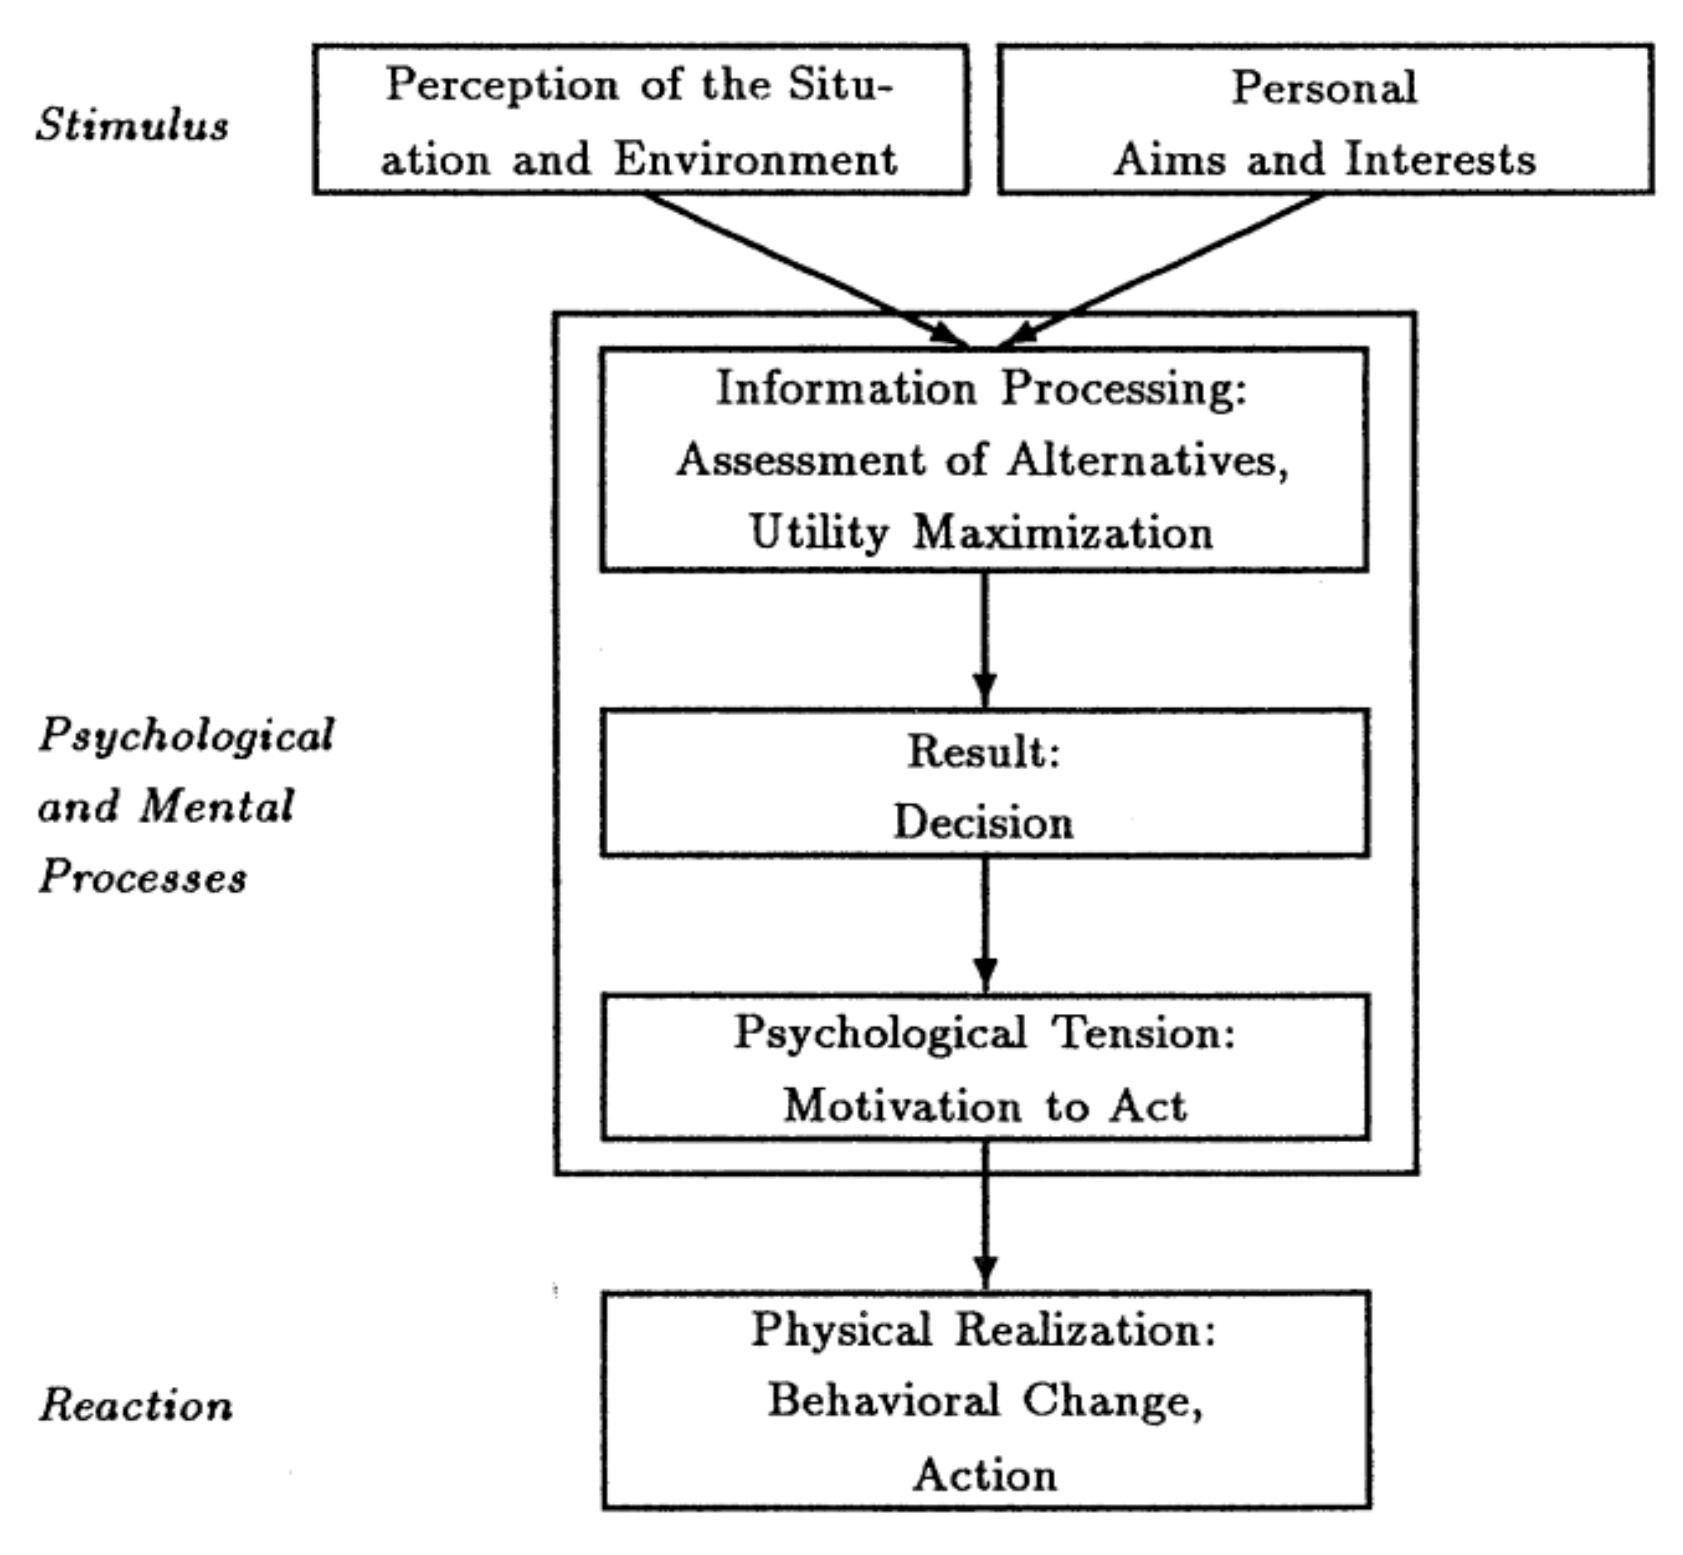
\includegraphics[width=1\linewidth]{images/helbingSocialForceConceptScheme.png}
  \caption{sequence of actions in the social force concept, taken from \protect\cite{helbing_social_1995}}
  %\Description{sequence of actions in the social force concept}
  \label{fig:helbingSchema}
\end{figure}
Fig. \ref{fig:helbingSchema} shows the sequence of actions leading to an action for an individual crowd agent based on research done by Lewin \cite{lewin_field_1951}. The Stimulus is used as a trigger like someone blocking the way for instance. This results in the process of handling the situation which creates a motivation to act and in the final form a reaction that is carried out. While this concept can be applied to all situations, Helbing however describes a model for common situations which are decided usually automatically and intuitively by the person. The idea is to describe the pedestrian movement indirectly through describing the external forces which affect the agent. 
Helbings social force model uses 3 main effects for the model:
\begin{enumerate}
    \item the goal for the person is to reach some sort of target destination as easy as possible, usually the fasted route.
    \item "repulsive effect": the pedestrian wants to "keep a certain distance from other pedestrians that depends on the pedestrian density and the desired speed". In addition the pedestrian also want to keep distance to borders.  
    \item "attracted effect": the pedestrians are sometimes attracted by other persons (friends, street artists, etc.) or objects (e.g., window displays)."
\end{enumerate}
In the paper all effects are described in detail with mathematical equations which are not displayed here for reasons of clarity. The resulting movement decision is the sum of all effects plus a fluctuation term for situations where two alternatives are rated equally. Simulations with this model show:
\begin{quote}
    "(i) the development of lanes consisting of pedestrians who walk into the same direction and (ii) oscillatory changes of the walking direction at narrow passages."
\end{quote}
This behaviour can also be observed in real world scenarios. 

\subsubsection{Simulating dynamical features of escape panic}\cite{helbing_simulating_2000} At the same time there is also a need for simulating pedestrians in a panic situation, a common example being evacuation simulations.
There are a number of reasons for a panic reaction in a crowd: unexpected actions like a loud gun shot or a fire are common reasons most people would think about. But also expected situations like the race for a limited amount of resources (tickets, seats, toilet paper during the COVID-19 pandemic)  and even situations without any cause at all can cause a crowd panic. These panic reactions often lead to tragic events and cause harm to people as seen for example in the panic at the loveparade 2010 \cite{dumbs_massenpanik_2010} . These events also show that the reaction of the individual agent is way more complex in a panic situation than under normal circumstances. This, of course, makes the development for a crowd behavioural model difficult. In addition the paper also states that there is not enough suitable data to test their panic model as they obviously can't simply produce a panic in the real world. 

The paper gives a definition of features of a panic situation, some of which are (1) People move faster than normal (2) People start pushing and so on. The full list is described in the paper. They use these features to construct a behaviour model based on the "generalized force model"\cite{hindsley_investigation_1986}
\begin{quote}
"We assume a mixture of psychological and physical forces influencing the behaviour in a crowd"
\end{quote}
They also ran a number of different tests with the model, the results showing the following:
\begin{itemize}
\item "Transition to in-coordination due to clogging": In a situation where the crowd wants to exit an area trough a small gap the number of people leaving gets smaller when the velocity of the crowd increases.
\item "Faster-is-slower effect due to impatience": Clogging can also appear when there is a wider gap in the escape route. 
\item "Mass behaviour": Here the goal was to leave a room with smoke in it. Results showed that the quickest evacuation would be possible when there is an equal mixture of individualistic and herding behaviour. 
\end{itemize}
In their model they have a "panic parameter" \label{term:panicParameter} which allows to adjust the "amount" of panic in comparison to a normal daily situation. Because the results are also observed in real crowd panics their model is often used as a base for a number of other evacuation simulation papers. \cite{braun_simulating_2005} \cite{zheng_modeling_2009}

\section{Application Areas}

As the research field for crowd simulation is already widely spread over multiple science fields and communities the resulting application areas are of course too. The applications can be roughly grouped by the key areas mentioned before \ref{chap:key_areas}. 

\subsection{realism focused simulation}

In the area of realism focused simulation pedestrian and traffic simulation plays a big role, as these are used to simulate large urban areas. There are a number of commercial available software for similar use-cases like simulating the crowd flow at events, in public transport buildings, airports and even cruise ships and whole city districts. They often come with extended features that go beyond the crowd simulation like heat-maps, smoke simulation, integration for 3D models and other CAD applications, recording and playback and so on. The customers for these applications are public transport companies, architectural offices, event organizers and the public governance sector. The simulation allows them to reduce costs in the planning phase and optimize their infrastructure. Simulation of the evacuation times required is also a market for these applications. Some example applications are "Pedestrian Dynamics®" \cite{pedestrian_dynamics_pedestrian_2020}, "MassMotion"  \cite{mediaworks_pedestrian_2020} and "Anylogic" \cite{anylogic_website}

\begin{figure}[h]
  \centering
  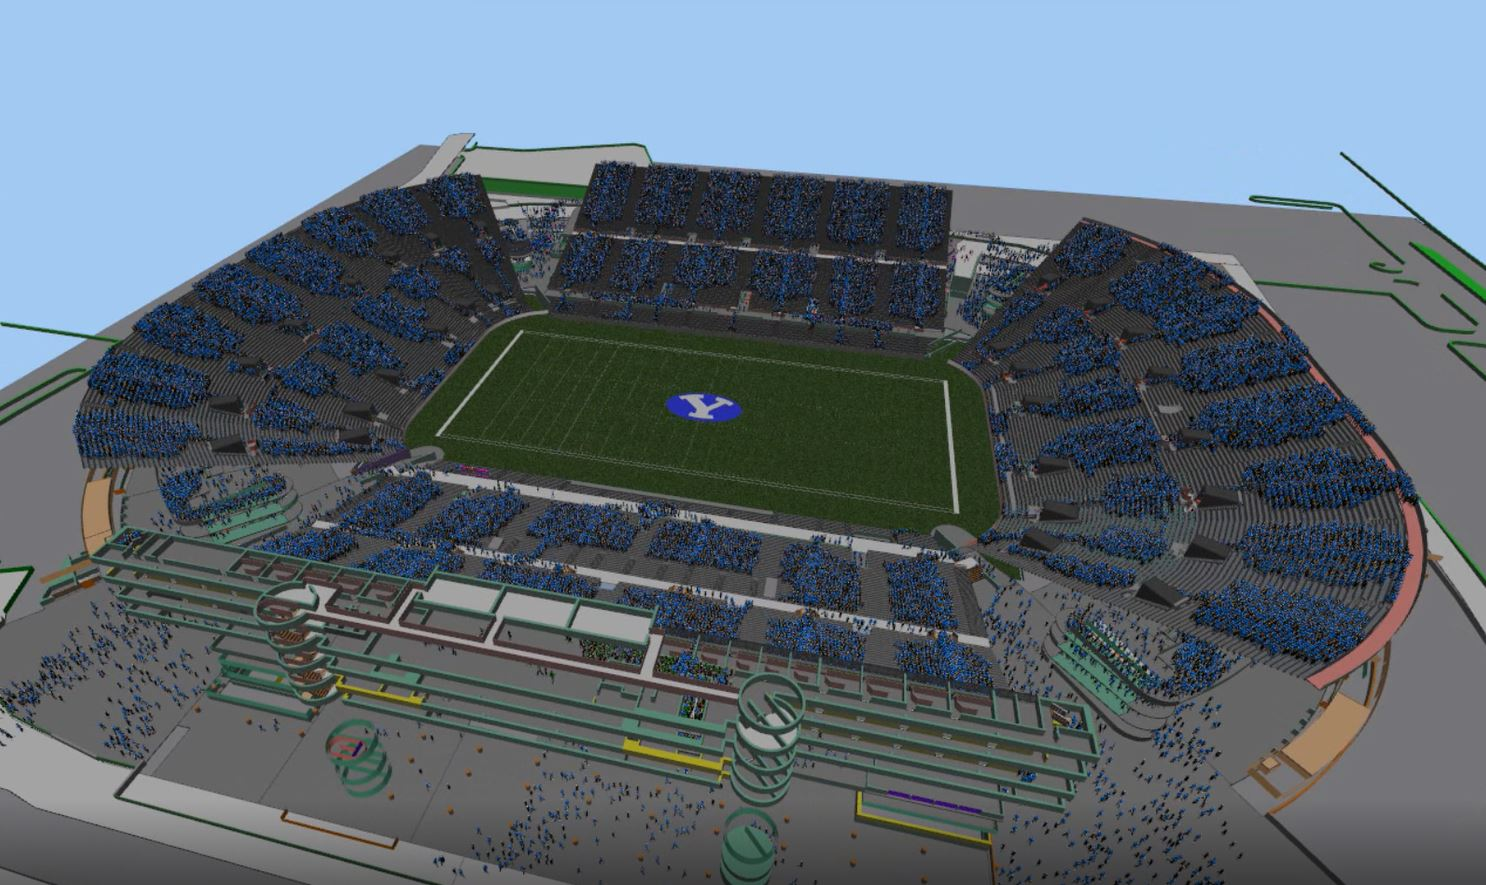
\includegraphics[width=1\linewidth]{images/PedestrianDynamicsStadionExample.png}
  \caption{example visualization of pedestrian flow in the commercial software "Pedestrian Dynamics®",  taken from \protect\cite{pedestrian_dynamics_pedestrian_2020}}
  %\Description{example visualization of a pedestrian flow in a stadium}
  \label{fig:stadionEvacuationExample}
\end{figure}
Although the visual presentation is not the focus of these applications it does not necessarily have to look basic. As some of the introduced commercial tools also have export functions for the generated behaviour, especially the movement, these exports can then be used later to produce visually appealing videos in 3D applications like "3ds Max" as a demo of Jordan Lynam shows us. \cite{lynamJordan_viissim_3ds_max}

\subsection{High quality focused simulation}

Meanwhile we have the visual focused applications. In comparison to the realism focused simulation applications publicly available applications and research are rare and hard to find. The reason for this is these, especially the applications used for movies, are highly proprietary and not published. Most of the time information is only available in the form of making-of documentaries, interviews and CGI trailers. 
However, the foundation these applications are based on is usually publicly available in the form of scientific papers. The challenges these applications are confronted with are strongly influenced by the crowd rendering research field, especially in games as these require real-time simulations. \cite{thalmann_crowd_2013}

\subsubsection{Movies}

There are multiple benefits of crowd simulation for movies and other types of creative video content. A nearly endless amount of possible scenes and shots can be created, for example a huge battle or a populated city. Some scenes would just not be possible to be animated manually with CGI not to mention hiring an amount of actors and actually filming it. In comparison to the realism focused applications, simulations for movies does not have the strong urge of proper continuous crowd behavior, as movies are grouped in shots where the viewer often doesn't see the same part of the crowd for a longer period of time. Lastly, creative content obviously doesn't always want realistically behaving crowds. Animators see crowd simulation more as a tool for controlling large crowds, so the research field for manipulation of crowds is also an important aspect on movie crowd simulation,  examples are \cite{kim_interactive_2014} \cite{ulicny_crowdbrush_2004}

In the recent movie "THE HOBBIT: Battle of Five Armies" there were  two types of crowd simulation tools used. "Massive", one of the most advanced non-real-time simulation tools \cite{massive_website} for rendering the final scenes in post production, which at this scale requires render farms to run for weeks or even months to finish. Therefore a second tool, "army-manager" was used earlier in the production, as this could render much faster and allowed the visual effects team to plan their shots and get a draft of the final simulated crowd. \cite{wired_hobbit_doku}

On the example of the movie "World War Z" we can also see that the simulations are often combined with a database of motion captures scenes. We already saw that approach in some literature \cite{thalmann_crowd_2013}, and rigid body physics. In addition the "Alice" program, which is used to simulate the zombie crowds, uses a microscopic based model where each agent is simulated by given rules and attributes, which we already know from a lot of papers. \cite{wired_worldwarz_doku} 

An other commercial software for CGI crowds is "Golaem" \cite{golaem_website}. This software can be purchased for individual projects and is therefore used for movies with a smaller budget, commercials or other short CGI clips in need for crowds, that can't afford to develop their own software tool, but it is also used for big budget productions for example in "Game of Thrones" \cite{golaem_got_vid}

\subsubsection{Games}

As games and other interactive media are real-time simulations they have limited capabilities for costly simulations, so crowd simulations are not so common in today's games. One game genre that uses them are real-time strategy games like Total War \cite{total_war_website}, where the crowd simulation can also have an effect on gameplay and is not only used to render visually appealing large crowds. 
Many approaches for real time simulation are using the common LOD (level of detail) technique for the rendering of the crowd and also for the simulation itself. However LOD is more complex when used on the actual crowd behaviour simulation than on the crowd rendering itself. There is always the danger of getting a wrongly simulated world when the simulation detail level is too low. Another commonly used trick is to render one simulated agent as multiple persons to simulate a crowd. Lastly, as games are usually run on a powerful GPU, real time crowd simulation can also benefit from that, especially the rendering part is well manageable by the GPU. \cite{thalmann_crowd_2013}

An example of what can be done with various optimization is "Ultimate Epic Battle Simulator" \cite{ultimeEpicBattleSim_video} , which is basically a big real-time crowd simulation sandbox. They manage to simulate path tracing on up to ten thousands of individual soldiers in real time. 
\begin{quote}
"The algorithm is a highly optimized version of A*.  \label{term:A*Usage} The memory is shared, but the paths are not." \cite{ultimeEpicBattleSim_video}
\end{quote} This example shows that crowd simulation at games comes with a big trade off for performance. 

\section{Research Areas}

The rough separation of the research field described in \ref{chap:key_areas} can be extended for more detail. \cite{thalmann_crowd_2013}

\subsection{Crowd behavior generation}

An automated model that animates the crowd movement is the core component for crowd simulation. Here, the goal is that our agents do not need to be animated manually in regard to where to go and how to interact with each other. The creator of the animation only provides some goals, for example escape from the building, and sets parameters like the "panic parameter" see \ref{term:panicParameter}. We already talked about some important aspects of that field in \ref{chap:simulationModels} and \ref{chapter:elementaryPapers}.  In this research area there are a lot of different approaches and the problem of application specific algorithms is bigger here than in other areas.

In the following I want to describe the different challenges we face in this area:

\subsubsection{Behavioral model}
We want a realistic crowd behavioral model for our specific use case that does not cost much performance and at the same time is adaptable so that the creator of the simulation is still able to control the crowd from a wider point of view. The model has to control how the individual agents gather in small groups and interact with each other. For example there can be multiple types of crowd agents: a leader, follower and people who want to walk alone are some examples which can be adapted for the application specific needs. Some example models here are \cite{musse_hierarchical_2001} for real time applications and \cite{braun_simulating_2005} for non real time evacuation applications. The selection of a model depends on the actual application and its individual needs.

\subsubsection{Crowd navigation}
This topic deals with the motion planning of a path from the beginning position to the goal position the agents have to reach in the long term. Some research here comes from the robotics field, as these share similar problem like \textbf{collision avoidance and path planning}. However, the algorithms have to be adapted for use in crowd simulations, as there are additional challenges like performance. To circumvent this, the path planning is done with abstract graphs, some of which are "grid graph", "point graph", "Navigation mesh / visibility graph", "Probabilistic roadmaps", "Rapidly exploring randomized trees" and "Voronoi diagrams". Afterwards graph search algorithms are run to plan the path to the goal. These include "Breadth-first search (BFS)",  "Depth-first search (DFS)", "Dijkstra’s algorithm", "A* algorithm" used in \ref{term:A*Usage} and hybrid approaches. A detailed overview for the mentioned graphs and algorithms can be found in the state of the art report of \cite{jaros_crowd_2014}. 

\subsubsection{Collision avoidance}
Collision Avoidance algorithms have to be used to prevent collisions between the dynamic environment (cars, collapsing building) and the individual agents and each other. The challenge is that we don't know at what velocity and in which direction each collision object will move in the future, and communication is usually not possible. A common approach is to predict the future movement through extrapolation \cite{karamouzas_predictive_2009}. Another would be to use vision-based approach \cite{ondrej_synthetic-vision_2010}.

\subsubsection{Additional behaviors}
For a realistic looking crowd there are often more animations than the core walking animation needed. Some papers for example research gaze animations and eye movement. 

\subsection{Generation of individual agents}
To simulate a realistic crowd it is necessary to have different 3D models to display in our crowd. The goal in this area is to develop methods which reduce the cost of time to create such models. There are multiple approaches over which I want to give a quick overview. Which approach to choose depends on multiple aspects like quality needed, amount of time that can be invested, what type of agents to produce (persons, cars, ...) and many more. 
\subsubsection{manually model agents}
The most basic way is of course to model each agent manually. The challenge is to also keep the polygon count low as this is required later on when we want to render the crowd. Techniques like subdivision modeling and patch modeling are used to achieve that.
\subsubsection{reconstruct from existing data}
Another approach is to use already existing data in the form of videos, a photo series or a 3D Scan from agents we want to simulate. Hole filling, noise reduction and skeleton hierarchy approximation are some challenges this approach faces in the process of finalizing the models. 
\subsubsection{interpolate existing models}
In some cases there are already models available to use. Of course these can also come from the approaches mentioned before. We can use these models to interpolate between multiple models to create new ones. Some papers also construct a template agent which can be used to generate models with given parameters (height, body type, ...)
\subsubsection{auto generated models from population}
An optimum would be to generate a large amount of diverse looking agents with as little information as possible, this idea being the goal for this approach. However, it is rather hard to create models that can compete against models from other approaches. One promising approach is the "somatotype model". It uses multiple extreme somatotypes and tries to generate models in between them. The demand for efficient result analysis to evaluate the generated models is another challenge. This is done with microscopic analysis, for testing the appearance against the input data, and macroscopic analysis for testing the diversity of generated models. 
\subsubsection{computer vision}
Is also another approach to generated customized models. This allows the user to generate a model based on an image. It is used in some games in the character creation process. 
\subsubsection{vary model for large crowds} 
One problem with all approaches is that they only work for a limited amount of agents effectively. To prevent the use of nearly similar looking agents and to reduce the memory needed for storing and later also rendering the agents it is possible to vary the generated models. This can be done on multiple levels like skeleton, meshes, textures and animations. 
\cite{thalmann_crowd_2013}

\subsection{Crowd animation}

After the generation of different models for our crowd we want to bring some life to it by utilizing animation. Some aspects we have to consider when creating animations are that they should not take much computational cost, be able to scale for a large amount of actors, allow level of detail gradation and provide a diverse select of possible matching. The animation consists of primary an secondary movements. When we take a person walking animation as example the actual walking would be the primary and other movements like hand gestures or phone interaction the secondary.
A often used approach is the use of an animation database, that is precalculated and can be used in the simulation later on. The database can be filled using locomotion cycles with procedural modeling or with motion capture of real animations. In the case of motion capture, a statistical model can be calculated which allows the production of a locomotion model. For more details see \cite{thalmann_crowd_2013}

\subsection{Interaction with virtual crowds}

Another area is researching how information from real crowds could be used to optimize the crowd behavior for virtual crowds. In the basic form people are observing real crowds and evaluate these results empirically to detect common patterns. These found patterns are later tried to be generalized in the form of individual, group and sociological aspects that can be implemented in the behaviour models of applications to provide accurate representation of the real world. To the individual aspects count behaviors such as personal/individual space and communication between individuals. Social conventions, group formation and leader selection are examples for group aspects. Sociological aspects describe behavior between a group and individuals, polarization, domination and the loss of individuality are some examples.  

In addition the automatic information gathering using computer vision is also part of this research field. The benefit of using these techniques is that first it is way less time consuming than manual observation and second that the infrastructure needed is quite cheap and often already available in the form of security cameras on public places. The information extraction is not just limited to person movement. A simple motion capture for the use in animation is also possible, or detection of events and their reactions, for example the persons reaction when a train is entering the platform. One example pipeline \cite{thalmann_crowd_2013} presented could be 1) extract trajectory for every person 2) group trajectories into "motion clusters" 3) compute an velocity field for each cluster 4) use these velocity fields in the virtual crowd simulation. 

\cite{thalmann_crowd_2013}

\subsection{Crowd rendering}

This area mainly deals with the technical details on how to render a large amount of individual agents. Especially in real time applications this is a big challenge. In addition, the quality of the agents also have to match the application, storage and data have to be managed efficiently and lastly our process has to be adaptable to different environments and situations. 
\cite{beacco_survey_2016} provides an good overview of the common used approaches dealing with these problems. They pointed out "that the rendering process is strongly tied to the simulation process and also to animation computations.". So to render a crowd in real time the other steps also have to be efficient enough to be calculated in real time.  

An important and often used approach is to use different levels of detail (LoD) for our final rendering, we already saw that approach in the form of simulation detail levels.\cite{osullivan_levels_2002}. However the goal of LoD in crowd rendering is to render different agents with different detail representations based on the importance of the agent in the current rendering frame. Usually the different levels are prepared beforehand and the decision what level to use is made at runtime. For character crowds, polygon based approaches are usually used which use multiple 3D models. Other techniques for LoD are point-based, where agents far in the distance are only represented as a point and therefore don't require any geometry, and image-based also known as impostors, use simple primitives with textures to fool the viewer. The primitives can be a simple billboarding technique or more complex shapes. In a complete application there will usually be a hybrid approach which combines multiple LoD techniques. The challenge here is to prevent flickering when the LoD or technique switches. 

Additionally, crowd rendering can also benefit from other performance techniques used in other rendering areas that focus mostly on an optimum use of the GPU and current hardware features. View frustum culling is one of them, which allows to exclude some agents from the rendering in the first place as these are hidden by other geometry or aren't even in the camera view anyway. A special case in crowd rendering is that not only static geometry can block the sight to an object but also a large amount of agents in one place. Some other techniques are primitive instancing, palette skinning and key-pose caching.     
\cite{beacco_survey_2016}

\cite{thalmann_crowd_2013}

\subsection{Generation of environments for crowds}

Here the research is focused on producing areas for the crowd simulation. As most applications simulate people crowds around cities the automatic construction of urban areas is a big research topic. The research done here ranges from terrain modeling, plants-, lakes- and building placements over building floor plans and streets. It is important to remember that the generated environment also impacts our whole simulation (path planning, collision avoidance, behaviour model, ...). 
As modelling these often large areas manually requires a lot of time, the need for automatic or semiautomatic algorithms is big. A rough separation of these methods are reconstruction based and parametric based approaches. 
Aerial photos, 2D maps and laser profiler data is used to reconstruct real world environments. These applications are usually applied for historical cities. 
Meanwhile parametric methods do not focus on the accurate representation of already existing areas, instead they want to provide cities for specific use cases where the application can decide on the parameters. These later can be filled with the crowd. Another important aspect is that the environment has to be interactive, for example  crowd agents should be able to enter buildings.
\cite{thalmann_crowd_2013}

\section{concrete example papers}

In the last chapter I want to present some concrete example researches in the crowd simulation field. 

\subsection{HiDAC System}

The paper "Controlling Individual Agents in High-Density Crowd Simulation" \cite{pelechano_controlling_2007} is an interesting example because it combines multiple simulation models and algorithms to simulate a crowd in one system, which they call High-Density Autonomous Crowds (HiDAC) system. They focus on delivering a simulation that produces realistic crowds.
In addition, this papers also shows what aspects are to consider and how to design a simulation model.

The initial problem was that there was no simulation model which could handle high-density crowds realistically. They wanted to combine the advantages of rule based and social force based models without their disadvantages.

\subsubsection{architecture and goals}
HiDAC is an agent based or microscopic simulation \ref{def:microscopic models}, so there is no higher system which controls the flow of the crowd, each agent acting on its own.
Fig. \ref{fig:hidacArchitecture} shows the two main modules of the system. The high-level module is responsible for long term tasks like wayfinding by choosing attractor points for each agent. Other more detailed or spontaneous tasks are handled by the low-level module, like collision avoidance to other agents  within a bounded space.
\begin{figure}[h]
  \centering
  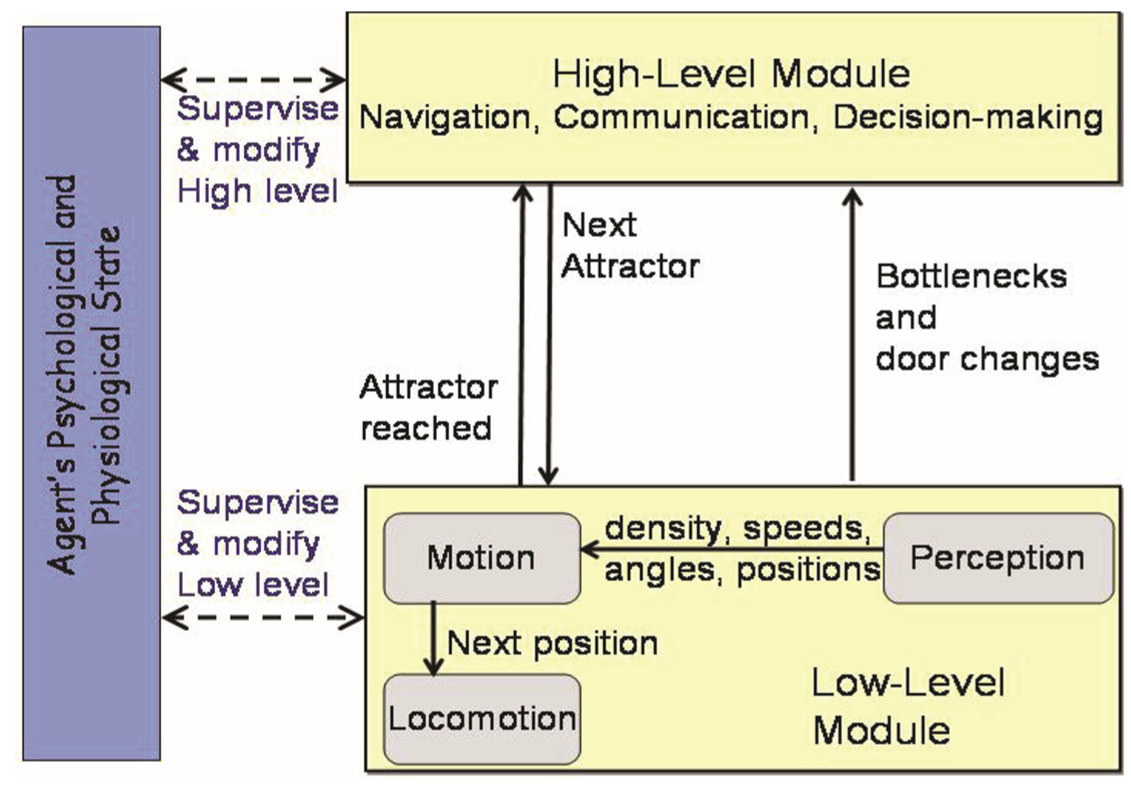
\includegraphics[width=1\linewidth]{images/hidac-architacture.png}
  \caption{architecture overview of HiDAC,  taken from \protect\cite{pelechano_controlling_2007}}
  %\Description{architecture overview of HiDAC}
  \label{fig:hidacArchitecture}
\end{figure}
For better performance and more realistic behavior the model separates the environment into different rooms that are connected by "portals" such as doors. Each agent chooses an attractor point in the room and navigates to it. Furthermore the agents only perform collision detection and other forces to agents in the same room, or in case the agent is in the area of a portal to other agents in the area of that specific portal.

The goals of the system are the following:
\begin{itemize}
    \item Preventing agents from appearing to vibrate (shaking behavior), which is often seen on social force based systems especially in high density areas or when an agent is in a hurry.
    \item Creating natural bi-directional flow rates. Other simulations often lack the behaviour of lane formation, which is however often observed in real crowds
    \item Queueing and other organized behavior
    \item Pushing through a crowd
    \item Agents falling and becoming obstacles 
    \item Propagating panic
    \item Exhibiting impatience
    \item Reacting in real time to changes in the environment
\end{itemize}

\subsubsection{solution}
To achieve these goals the papers presents a detailed calculation based on different forces and tricks. In the following I want to summarize the ideas of the model and calculation. 

As a starting point, they define a rectangle of influence for each agent, which is calculated based on the distance and angle to other static and dynamic objects. This allows to optimize performance, as only objects in the own rectangle of influence have to be considered for further calculations. 
There are three main forces: \textbf{avoidance force, tangential force and repulsion force}. Avoidance force prevents direct collisions with objects. It is applied to static objects and other agents. Tangential force happens between agents and is used to control agents in a situation where they run towards each other, these are called bi-directional flows. On high density crowds this force allows the simulation to create the realistic behavior of lane formation. Interestingly this is not explicitly implemented in the model but results from the applied forces. Lastly, the repulsion force is triggered as a result of a collision with a static object like a wall or another agent. The main difference is that agents, compared to walls, can be pushed away. 

In addition to the forces there are other tricks which allow them to boost their realistic simulation. 
A very important one is the \textbf{stopping rule}. Based on the personality and current situation an agent may stop moving for a given time before he continues walking toward its attractor, however the agent can still be pushed away. This rule solves the shaking problem which most social force models have, but still allows the realistic pushing forces on agents. 
A similar rule is the \textbf{waiting rule} that allows queues to be formed in non panic situations. Modeling of a different \textbf{personal space} for each agent allows the system to perform agents pushing each other. 
The systems also allows to simulate a falling agent as a static obstacle in the case of a very dense crowd and special behaviour in panic situations. 
The separation into different modules and communication between them allows the low-level module to detect bottlenecks and the high-level to find an alternative path, this is known as \textbf{crowd impatience}. Similar to this, rerouting in the case of a changing environment works, for example when a door is blocked.

\subsection{vision based system}

"A Synthetic-Vision Based Steering Approach for Crowd Simulation" \cite{ondrej_synthetic-vision_2010} present an approach to control a microscopic simulation without using any forces, instead relying purely on predictions based on the view for each agent.
But in comparison to HiDAC where a whole crowd simulation system was described, this approach only focuses on individually walking humans and their collision avoidance behavior. In addition, they explicitly do not focus on a high-performance solution, however there are some notes on possible performance improvements and benchmarks included. 

The basic idea is that each agent decides based on their own visual perception of the environment and other agents whether they can continue their path or need to make an adaption by turning or decelerating. There are similar approaches in the robotics field, but these use image processing to get the information needed. Their system directly computes the visual image using 3D graphics processing on the GPU.
The method they use does not explicitly check for collision instead it tries to minimize the chance of possible collision. The authors say that their approach using visual perception is better at imitating the real human locomotion control.

\subsubsection{model overview}

The model is based on research from Cutting "How we avoid collisions with stationary and moving objects", his results on how humans avoid collisions can be broken down into two questions: 
\begin{itemize}
\item Will a collision occur? This is decided by an angle to the obstacle named the bearing angle $\alpha$ . When the derivative of the angle \textbf{\.{$\alpha$}} is zero a collision will occur. Fig\ref{fig:visualBearingangle} visualized the bearing angle and when a collision occurs.
\item When will a collision occur? Using the rate-of-growth for obstacles humans can estimate the \textbf{time-to-collision (ttc)}
\end{itemize}
\begin{figure}[h]
  \centering
  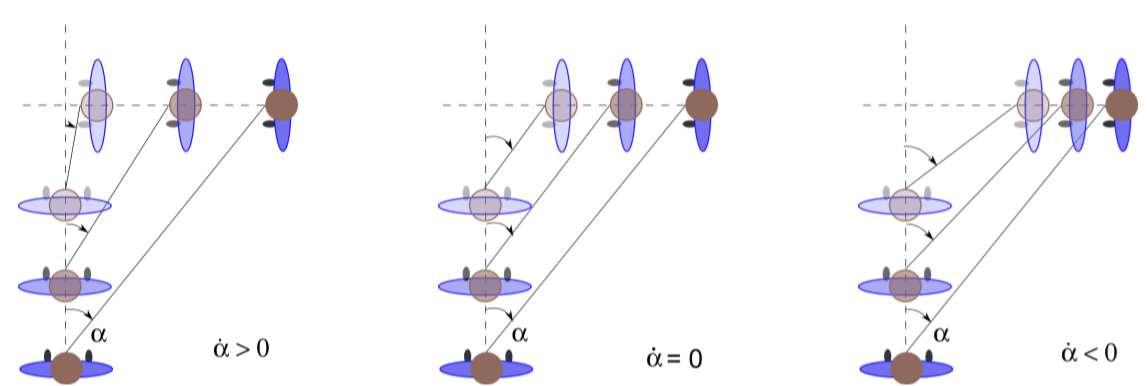
\includegraphics[width=1\linewidth]{images/visualApproach-bearingAngle.png}
  \caption{bearing angle and its time-derivative to detect collisions, taken from \protect\cite{ondrej_synthetic-vision_2010}. The picture in the middle will result in a collision therefore \.{$\alpha$} is zero}
  %\Description{bearing angle}
  \label{fig:visualBearingangle}
\end{figure}
The paper changes the use of time-to-collision to time-to-interaction tti, so the time needed before the two participants get closest to another this can be a collision or just a walk by. So in conclusion the information when and where two agents get the closest to another and if a collision will occur can be described by the pair (\.{$\alpha$}, tti). As a general rule of thumb: turning changes \.{$\alpha$} and deceleration changes tti. 

\subsubsection{implementation of steering and collision avoidance} A simplified version for the algorithm can described as following (for every agent):
\begin{enumerate}
    \item a virtual camera is set up using OpenGL with the view of the agent. Each pixel point represents an perceived point where the calculation is performed. 
    \item based on the rendered image by the camera,the velocity and distance for obstacles and our own velocity we calculate the pair (\.{$\alpha$}, tti) for each perceived point.
    \item When \.{$\alpha$} is below a threshold and $tti > 0$ and also lower than a threshold then a change in direction for this perceived point is necessary. 
    \item the turning and deceleration information for each perceived point is combined into one metric 
    \item updating the position of the agent using the calculated metric
\end{enumerate}

\subsubsection{results}

Fig \ref{fig:visualResults} shows the results from the simulation. The advantage of this approach is the realistic lane formation behaviour as well as correctly handling a circle situation. Smooth animations are generated because deceleration only occurs right before a collision happens. The simulation shows a visual appealing result however there is no confirmation if these results reflect the reality of crowds.

\begin{figure}[h]
  \centering
  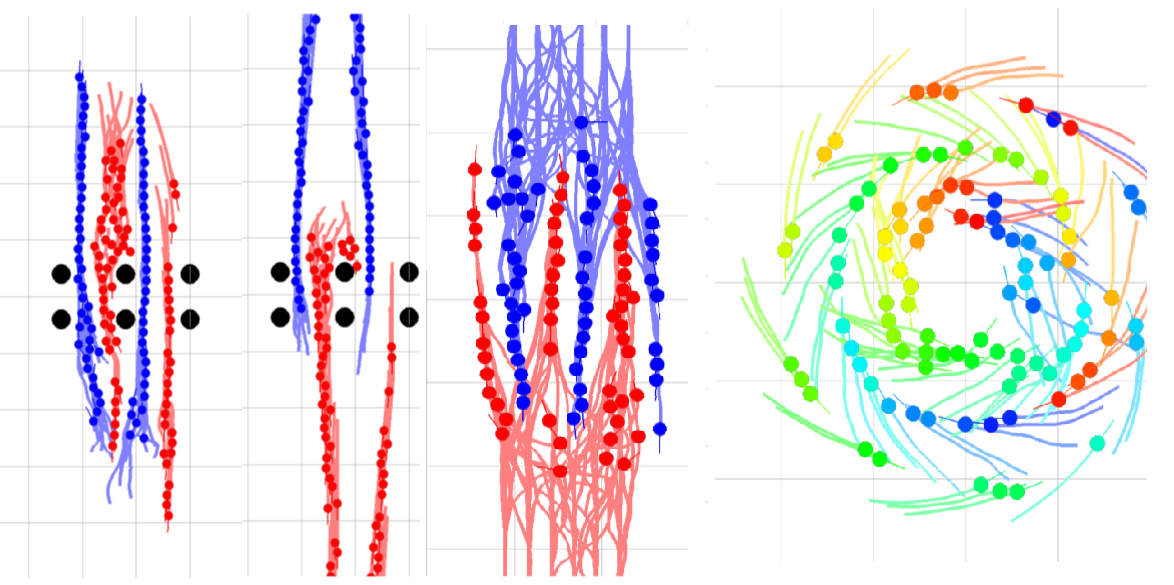
\includegraphics[width=1\linewidth]{images/visualApproach-results.png}
  \caption{results showing the lane formation  and traffic circles behaviour, taken from \protect\cite{ondrej_synthetic-vision_2010}.}
  %\Description{results}
  \label{fig:visualResults}
\end{figure}

\subsection{ViCrowd}

The paper "Hierarchical model for real time simulation of virtual human crowds" \cite{musse_hierarchical_2001} presents a crowd simulation system named ViCrowd. 
The goal is to deliver a complete simulation system that can run in real time. 
There are multiple parts that make this paper interesting and stand out from others in the field. These parts I want to summarize here. 

\subsubsection{multilevel hierarchy}
The model they use is unique because it is a combination of a macroscopic and microscopic model. The goal here is to use the performance advantage of macroscopic models while keeping the advantages of individualism and the resulting realism of microscopic models.
They achieve this by taking the agents and assign them to different groups. As a result, there are three complexity levels: (1) the whole crowd, (2) the different groups, (3) the individual agents. Although the assignment to the group is not fixed and an agent can convert to a different group during the simulation, an agent is only assigned to one group at the same time.

Each level has a different complexity and assigned tasks / calculations. 
The simplest level is the agent level where only a small amount of the movement decisions are made. Collision avoidance in the local area is one of them, as this can't be done at the group level.
The most influential level is that of the group. Here the most knowledge is saved and complex decisions are made, for example path planning.
At the crowd level only information relevant for all groups are stored and processed, for example interest points of the scene.
The information flow is mostly top to bottom, so crowd$\rightarrow$group$\rightarrow$individual.
This separation of levels and complexity allows the system to reduce the number of complex tasks and reuse information for multiple individuals at a group level. The simulation gains a huge performance benefit while keeping most of the realistic behaviour of a pure microscopic model. 
\subsubsection{combination of autonomous and scripted behaviour}
ViCrowd provides three ways of handling group behaviour: autonomous, guided and programmed. 
Autonomous groups handle all their movement by themselves. Guided groups are controlled from an external controller in real time during the simulation. And programmed groups act at simulation time accordingly to their beforehand provided script. Users can define the crowd or group behaviour using the provided script language. At runtime the system assigns the scripts the to specific groups. 
What is interesting about this approach is that all three methods can be combined even on the same group. For example, the user can directly guide a group, but the individual agents still handle the collision avoidance. To manage this they implemented a behaviour priority model for the different input methods.
\subsubsection{crowd information}
As basis for decision-making ViCrowd uses three categories of information. Knowledge, beliefs and intentions. 
%%See Fig \ref{fig:hierarchicalInformationOverview} for an overview.
%%
Knowledge is about stored information about the real environment, position of obstacles etc. 
Belief is a set of behaviour and emotions individuals and groups share, for example flocking behaviour.
Intentions usually are at group and individual level only and consists of goals to achieve. Some examples are at group level interesting points and at individual level when to change to a different group.
%%\begin{figure}[h]
%%  \centering
%%  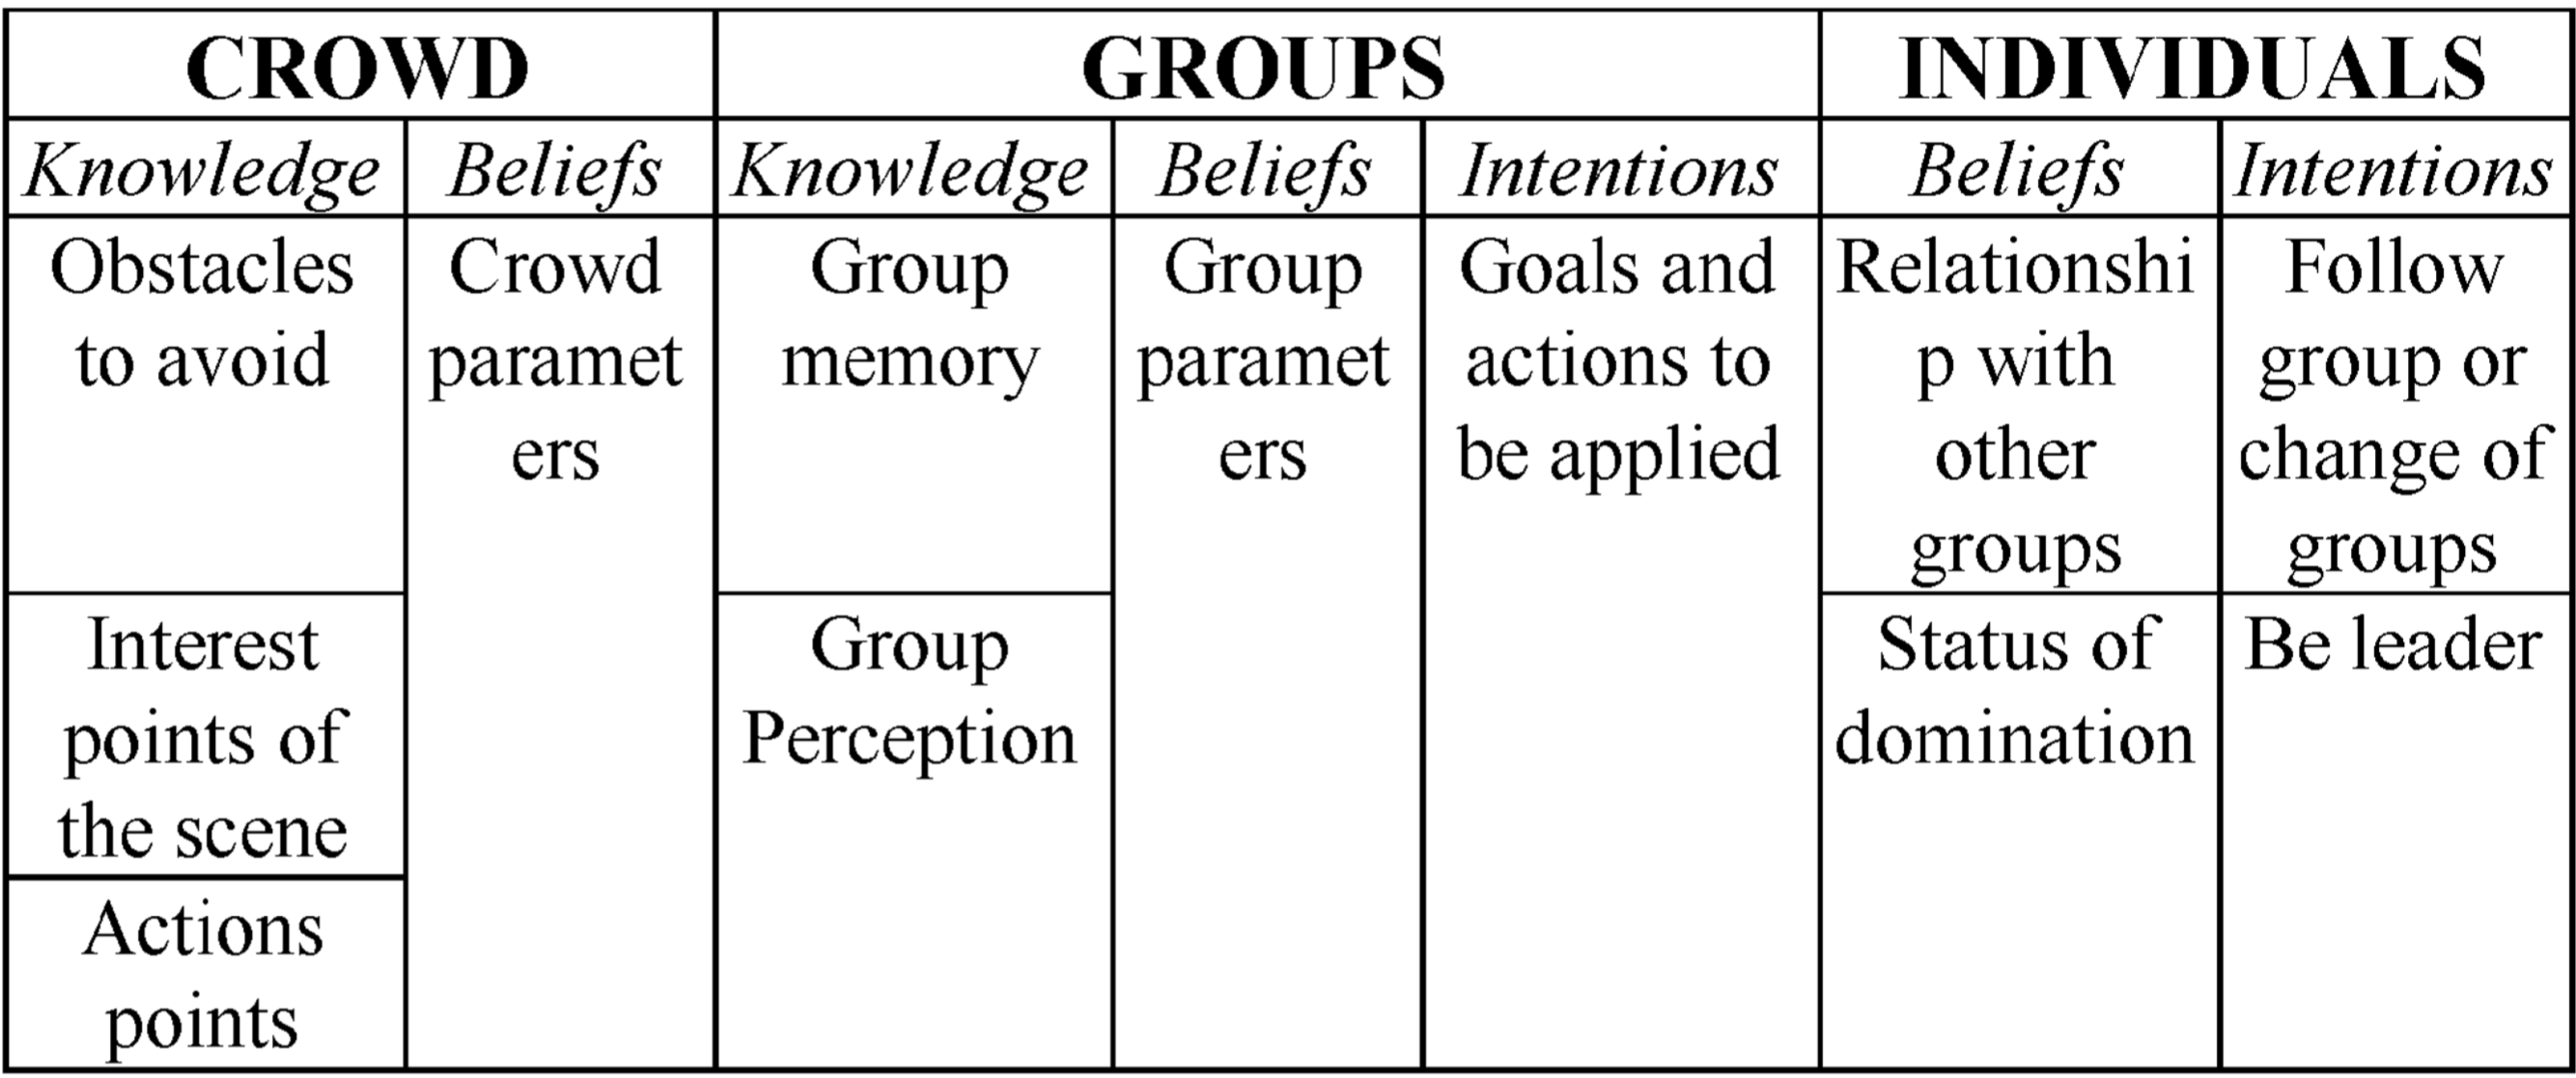
\includegraphics[width=1\linewidth]{images/HierarchicalCrowdInformationOverview.png}
%%  \caption{Overview of used information categories with examples, taken from \cite{musse_hierarchical_2001}.}
%%  \Description{information overview}
%%  \label{fig:hierarchicalInformationOverview}
%%\end{figure}
Fig. \ref{fig:hierarchicalarchitectureOverview} shows an overview of the complete ViCrowd system. The result is a low-level behavior for each group which is distributed to its assigned agents. The resulting pattern for each agent is similar to the other group members, but also includes their own details like local collision avoidance.

\begin{figure}[h]
  \centering
  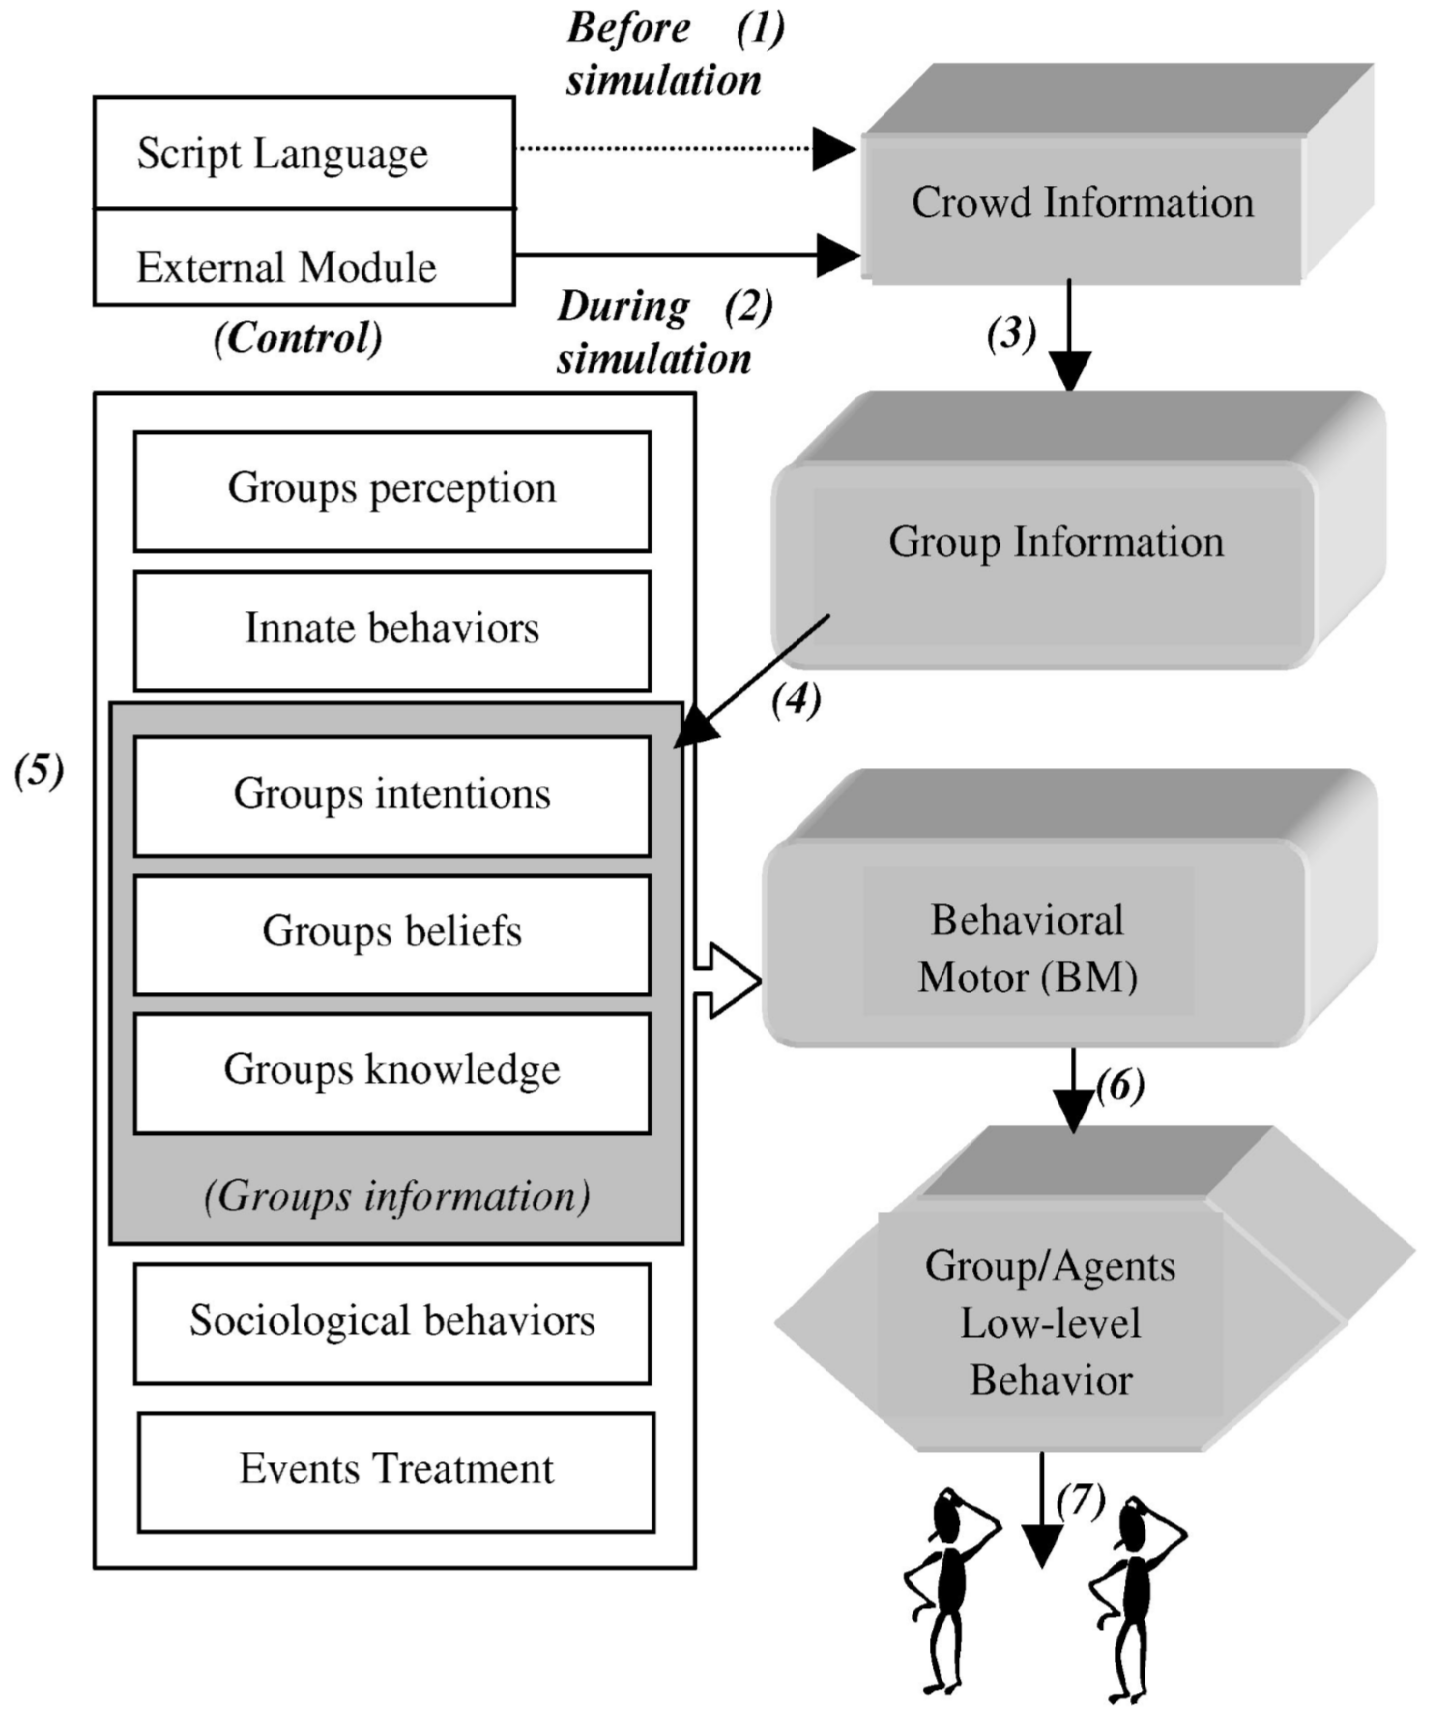
\includegraphics[width=1\linewidth]{images/HierarchicalArchitectureOverview.png}
  \caption{Overview of the architecture of ViCrowd, taken from \protect\cite{musse_hierarchical_2001}.}
  %\Description{architecture of ViCrowd}
  \label{fig:hierarchicalarchitectureOverview}
\end{figure}

\subsection{data-driven system}
"Crowds by Example" \cite{lerner_crowds_2007} have a completely different approach than other crowd simulation models. They simulate a crowd without the need for social rules or agents' perceptions. The system only relies on given input data in the form of videos from real world crowds.
However, there are multiple restriction and assumptions. First, they only focus on providing a mechanism for the steering aspect of agents, and second, the agents do not have a specific goal like reaching a point of interest.

The basic idea is to create a database of the steering behaviour agents in crowds have based on a given input of videos. At simulation time the system analyses the current situation and searches for a similar pattern in the database, then applies the steering behaviour of real humans in the database to the agent in the simulation. The advantages of this method are: 
\begin{itemize}
    \item The resulting animation offers a big diversity of steering behaviour, which results in a better visual appealing simulation.
    \item Because there are no explicit rules or assumptions about the crowd behavior the simulation is only dependent on the input data. This means that the system is not domain specific and can be adapted to different use cases by changing the input data.
\end{itemize}

\subsubsection{preparing the database}
The input data should consist of video clips filmed from a top perspective. In a second step the movement data needs to be tracked. In the example they tracked it by hand.
The system takes this tracked data and creates example trajectories, based on information such as the surrounding obstacles and other agents, which will be saved in the database. The influence function decides which aspects of the tracked data is used to create the examples. 

\subsubsection{running the simulation}
At the beginning of the simulation static obstacles like walls are placed. After that the environment is filled with agents that have a starting position and velocity. Then the simulation process begins.
The system checks in each simulation step for every agent if it needs to calculate a new steering trajectory. There are two question to consider for that: 
\begin{itemize}
    \item Has the agent already fulfilled the whole assigned trajectory?
    \item Has the surrounding environment changed since the last trajectory was assigned, for a defined threshold.
\end{itemize}
If the system needs to assign a new trajectory it creates a query with the given surrounding area, which is than performed against the database. As a result, the database gives us a most appropriate result trajectory that we assign the agent. 
However, the problem here is that collisions can occur. They deal with this by checking the trajectories for every agent if a collision will occur. If a collision is found the next best match from the database is used instead. If all matches fail to deliver a collision free simulation a fixed calculation tries to find a path away from the collision. 

\subsubsection{results}
In their example the database consists of thousands of examples. They use an approximate nearest neighbor search to find similar entries in the database, tough for the collision avoidance they use a simple brute force approach. In addition, finding the right parameters for the simulation was a challenge.
The resulting animation shows a variety of different steering behaviour and smooth collision avoidance without any problem of vibration.  
A big problem is the performance aspect: they only managed to do real-time simulation with two agents at 20 agents; the performance dropped to ~5fps. 
For future work a combination with a specific goal or a combination with other models is possible. In addition, the definition of the influence function and query can also be approved.

\subsection{ai-driven systems}
A relative new approach are ai-driven simulation system as "Crowd simulation by deep reinforcement learning" \cite{lee_crowd_2018} shows. They use reinforcement learning and deep neural networks (DNN) with a simple reward function to simulate the way finding and collision avoidance for each agent individually, so it is a microscopic process. In comparison to the other presented systems this paper only focuses on the aspect of agent navigation but each agent has a target destination in the simulation.

\subsubsection{model}
They simplify the simulation to a 2D area. Each agent has a radius $r$, a position $p$ and an orientation $\theta$, obstacles are modeled the same way except they don't have an orientation. 
This simplifies the collision detection, as this can easily be checked by measuring the distance between two simulation objects and comparing it to the sum of their radii.

For the reinforcement learning part they define the problem as a sequential decision-making or more specifically as a Markov decision process. For more details please directly check the paper. The basic idea is that the deep neural network tries to optimize the reward function. This again is defined by 
\begin{equation}
R = r_{goal} + r_{collision} + r_{smooth}
\end{equation}
where $r_{goal}$ influences the distance from the agent to the goal. $r_{collision}$ is a constant factor that is added, if an collision occurred, however, the number of collisions does not matter here. $r_{smooth}$ is a function to cover the smoothness of the movement by comparing the resulting position and orientation to their minimum and maximum values.  

\subsubsection{algorithm}
To get input data for the reinforcement learning they use visual sensors that act like casting rays from the center of the agent see Fig. \ref{fig:aiConceptOverview}. While the simulation is running, during every simulation step the system generates new values for the agents position and orientation based on the DNN. When the learning process is active it also influences the DNN through the reward function.
\begin{figure}[h]
  \centering
  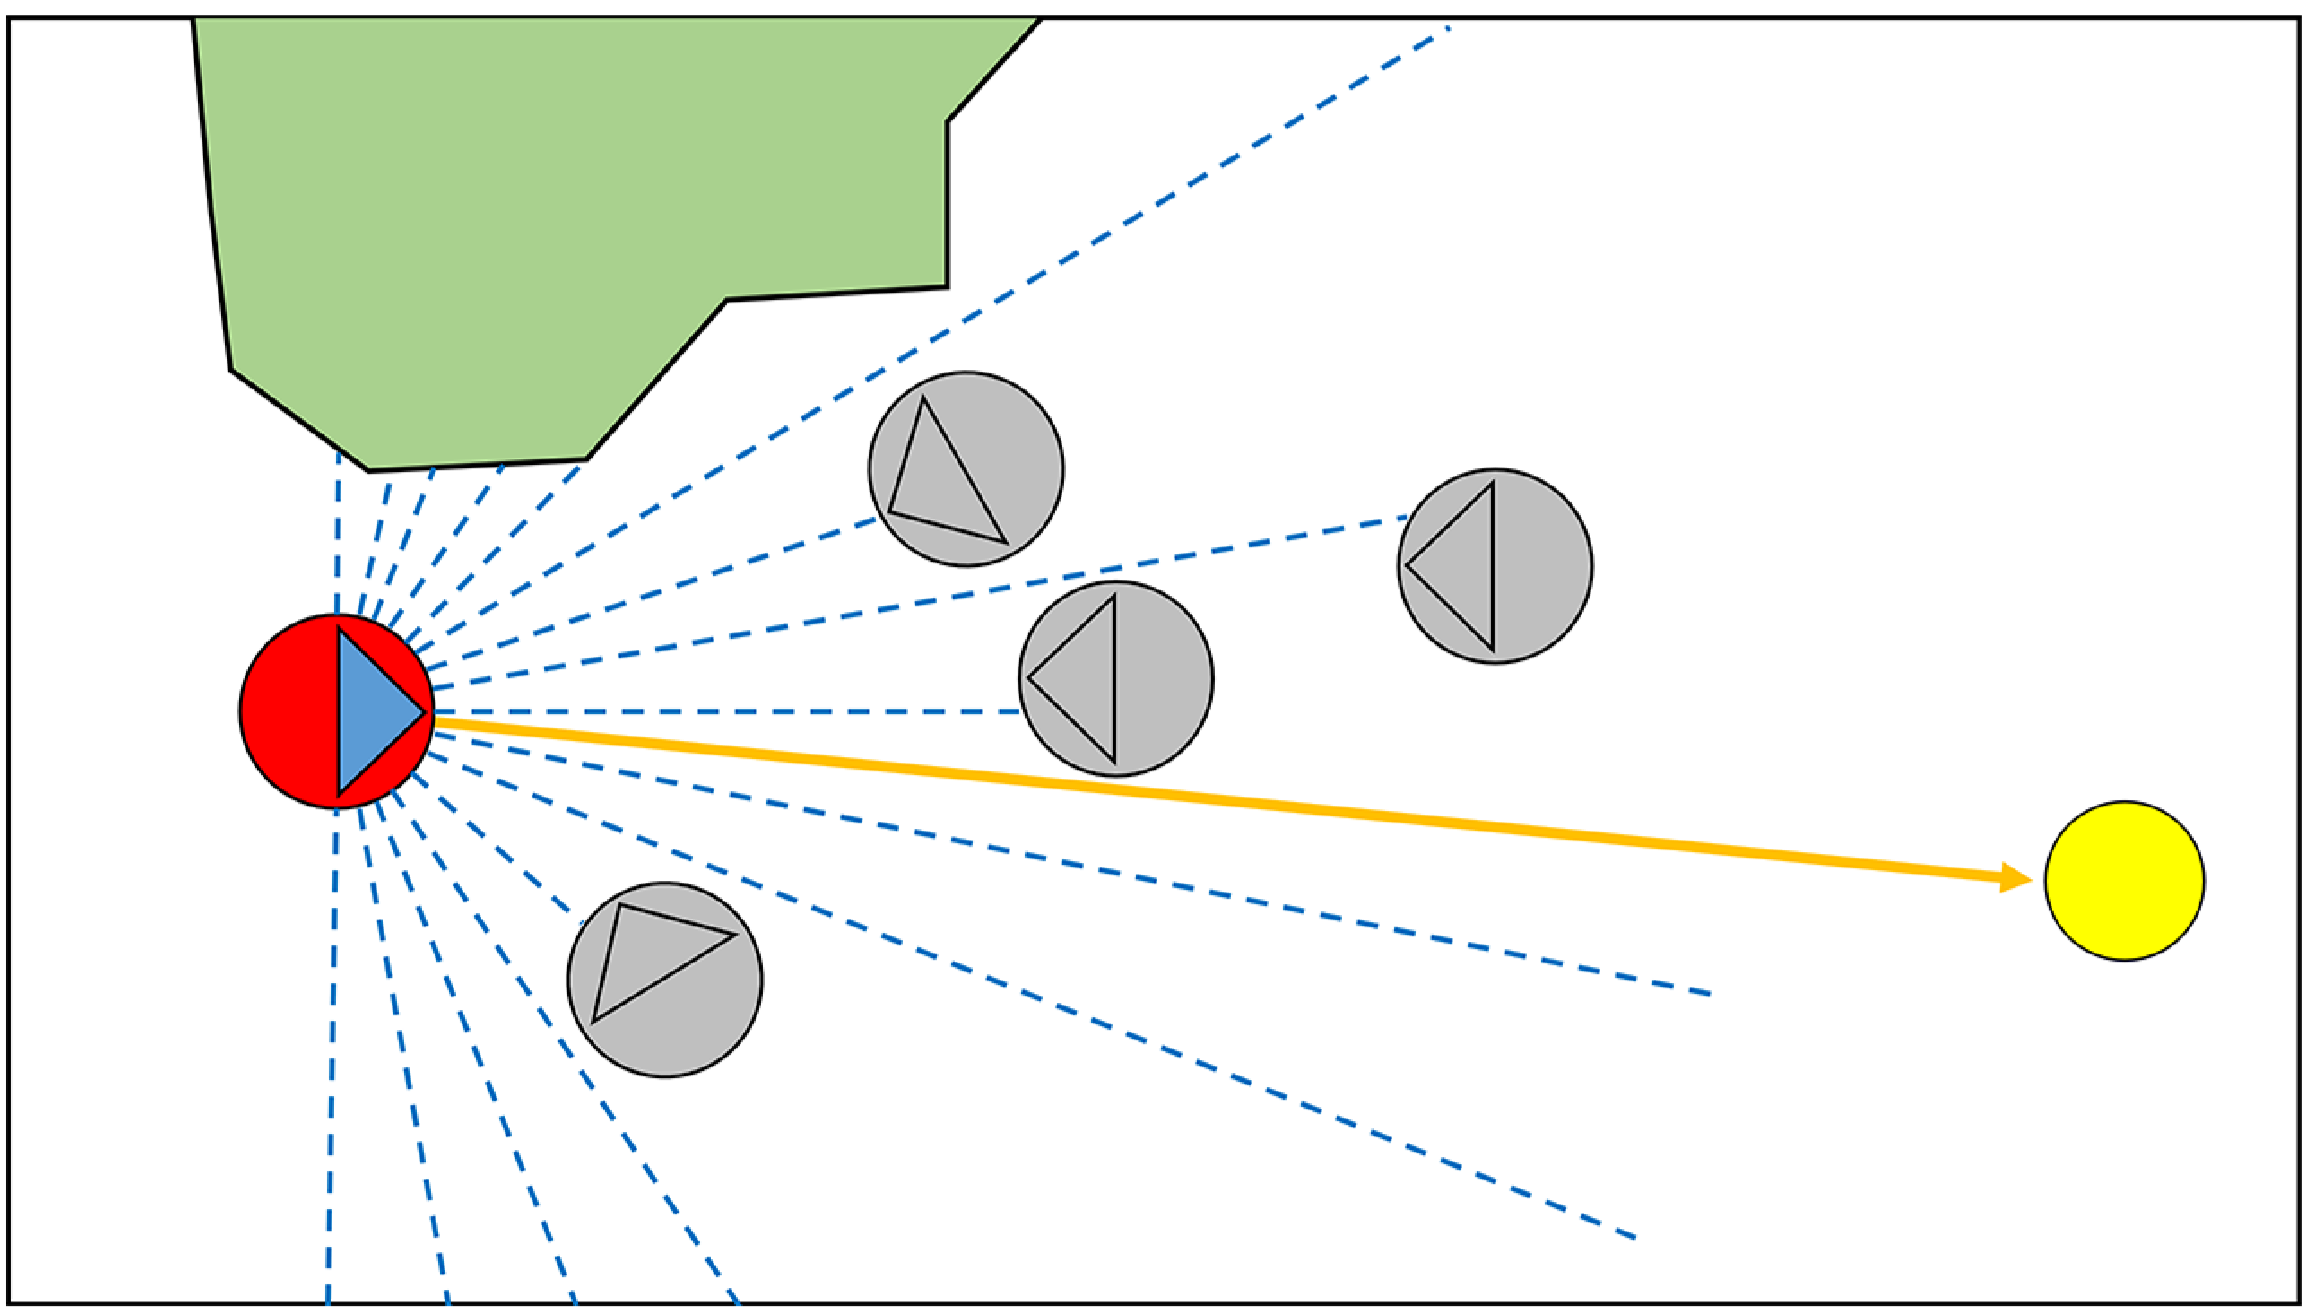
\includegraphics[width=1\linewidth]{images/aiAlgortihmn.png}
  \caption{Overview of concept idea, red dot represents the agent, yellow dot the goal, grey dots other agents and the blue line the visual rays for the calculation of the path, taken from \protect\cite{lee_crowd_2018}.}
  %Description{concept idea of the ai-driven system}
  \label{fig:aiConceptOverview}
\end{figure}

\subsubsection{results}
To test their system they run tests with 4 different scenarios, see Fig. \ref{fig:aiScenarios}. In a first step the system was trained for that specific scenario only, where they began with few agents and increased the complexity of the situation over time. Interestingly, the hallway scenario differs quite significantly as the learning curve only rises up late at ~45-50 thousand iterations, see Fig. \ref{fig:aiPerformance}.

After that they also ran tests for a generalizing DNN that works for all scenarios. To do that, they randomly selected different scenarios, preferring easier ones at the beginning. Their results show that a generalizing DNN can perform equally well compared to one specially prepared for that scenario. 

In conclusion that approach looks promising, as this requires relatively low effort in preparing the data compared to data-driven system, and still doesn't rely on any explicitly set behaviours. However, while the resulting simulation looks visually appealing but there was no validation if the resulting behaviour is also present in real world crowds. As for future work, they suggested to combine an ai-driven microscopic process with a multi-agent reinforcement learning one to gain the benefits of a macroscopic model. This would mean to adapt the reward function on multiple agents instead of treating each agent separately.  

\begin{figure}[h]
  \centering
  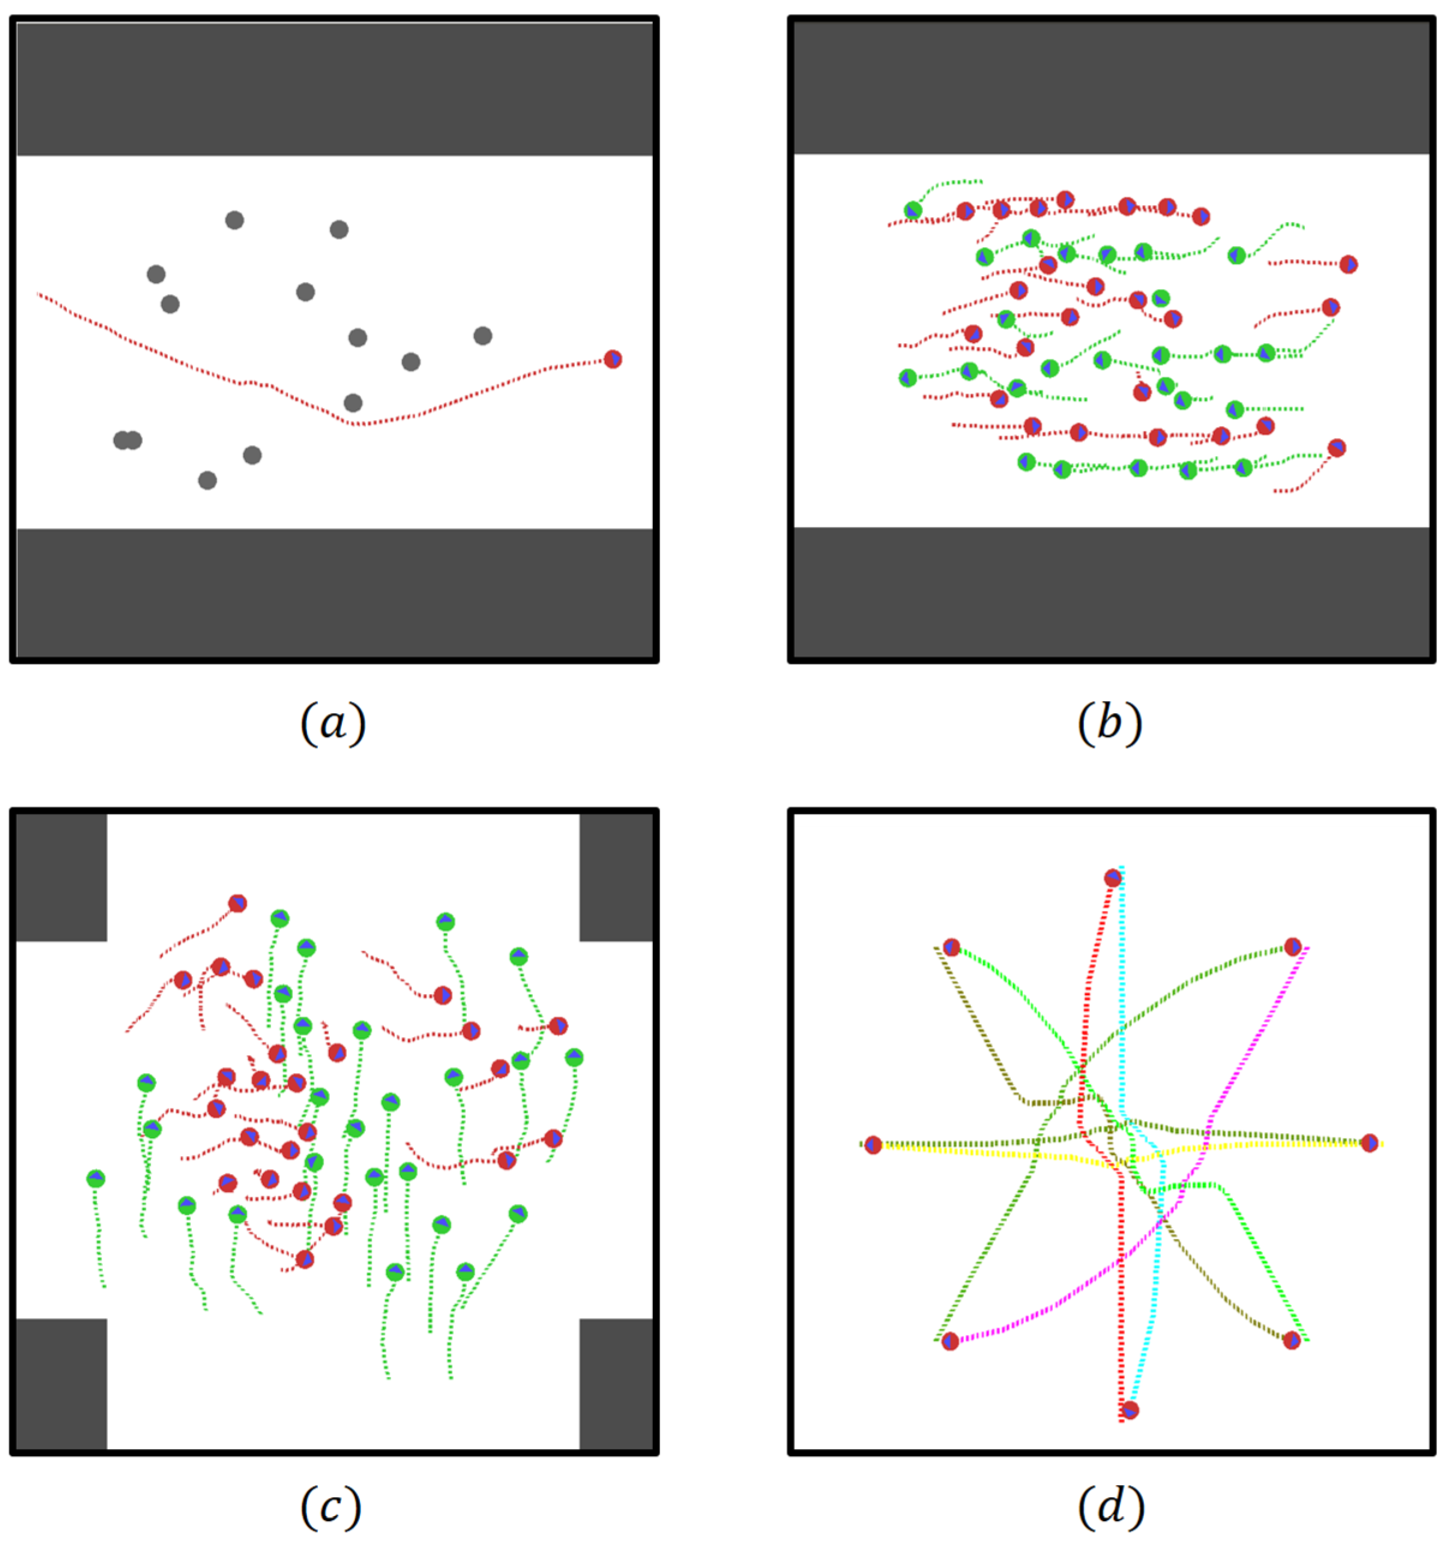
\includegraphics[width=1\linewidth]{images/aiSituations.png}
  \caption{Results of different simulation scenarios, (a) Obstacle (b) Hallway (c) Crossway (d)Circle  Graphs for specifics scenarios, taken from \protect\cite{lee_crowd_2018}.}
  %Description{Results for different simulation scenarios}
  \label{fig:aiScenarios}
\end{figure}

\begin{figure}[h]
  \centering
  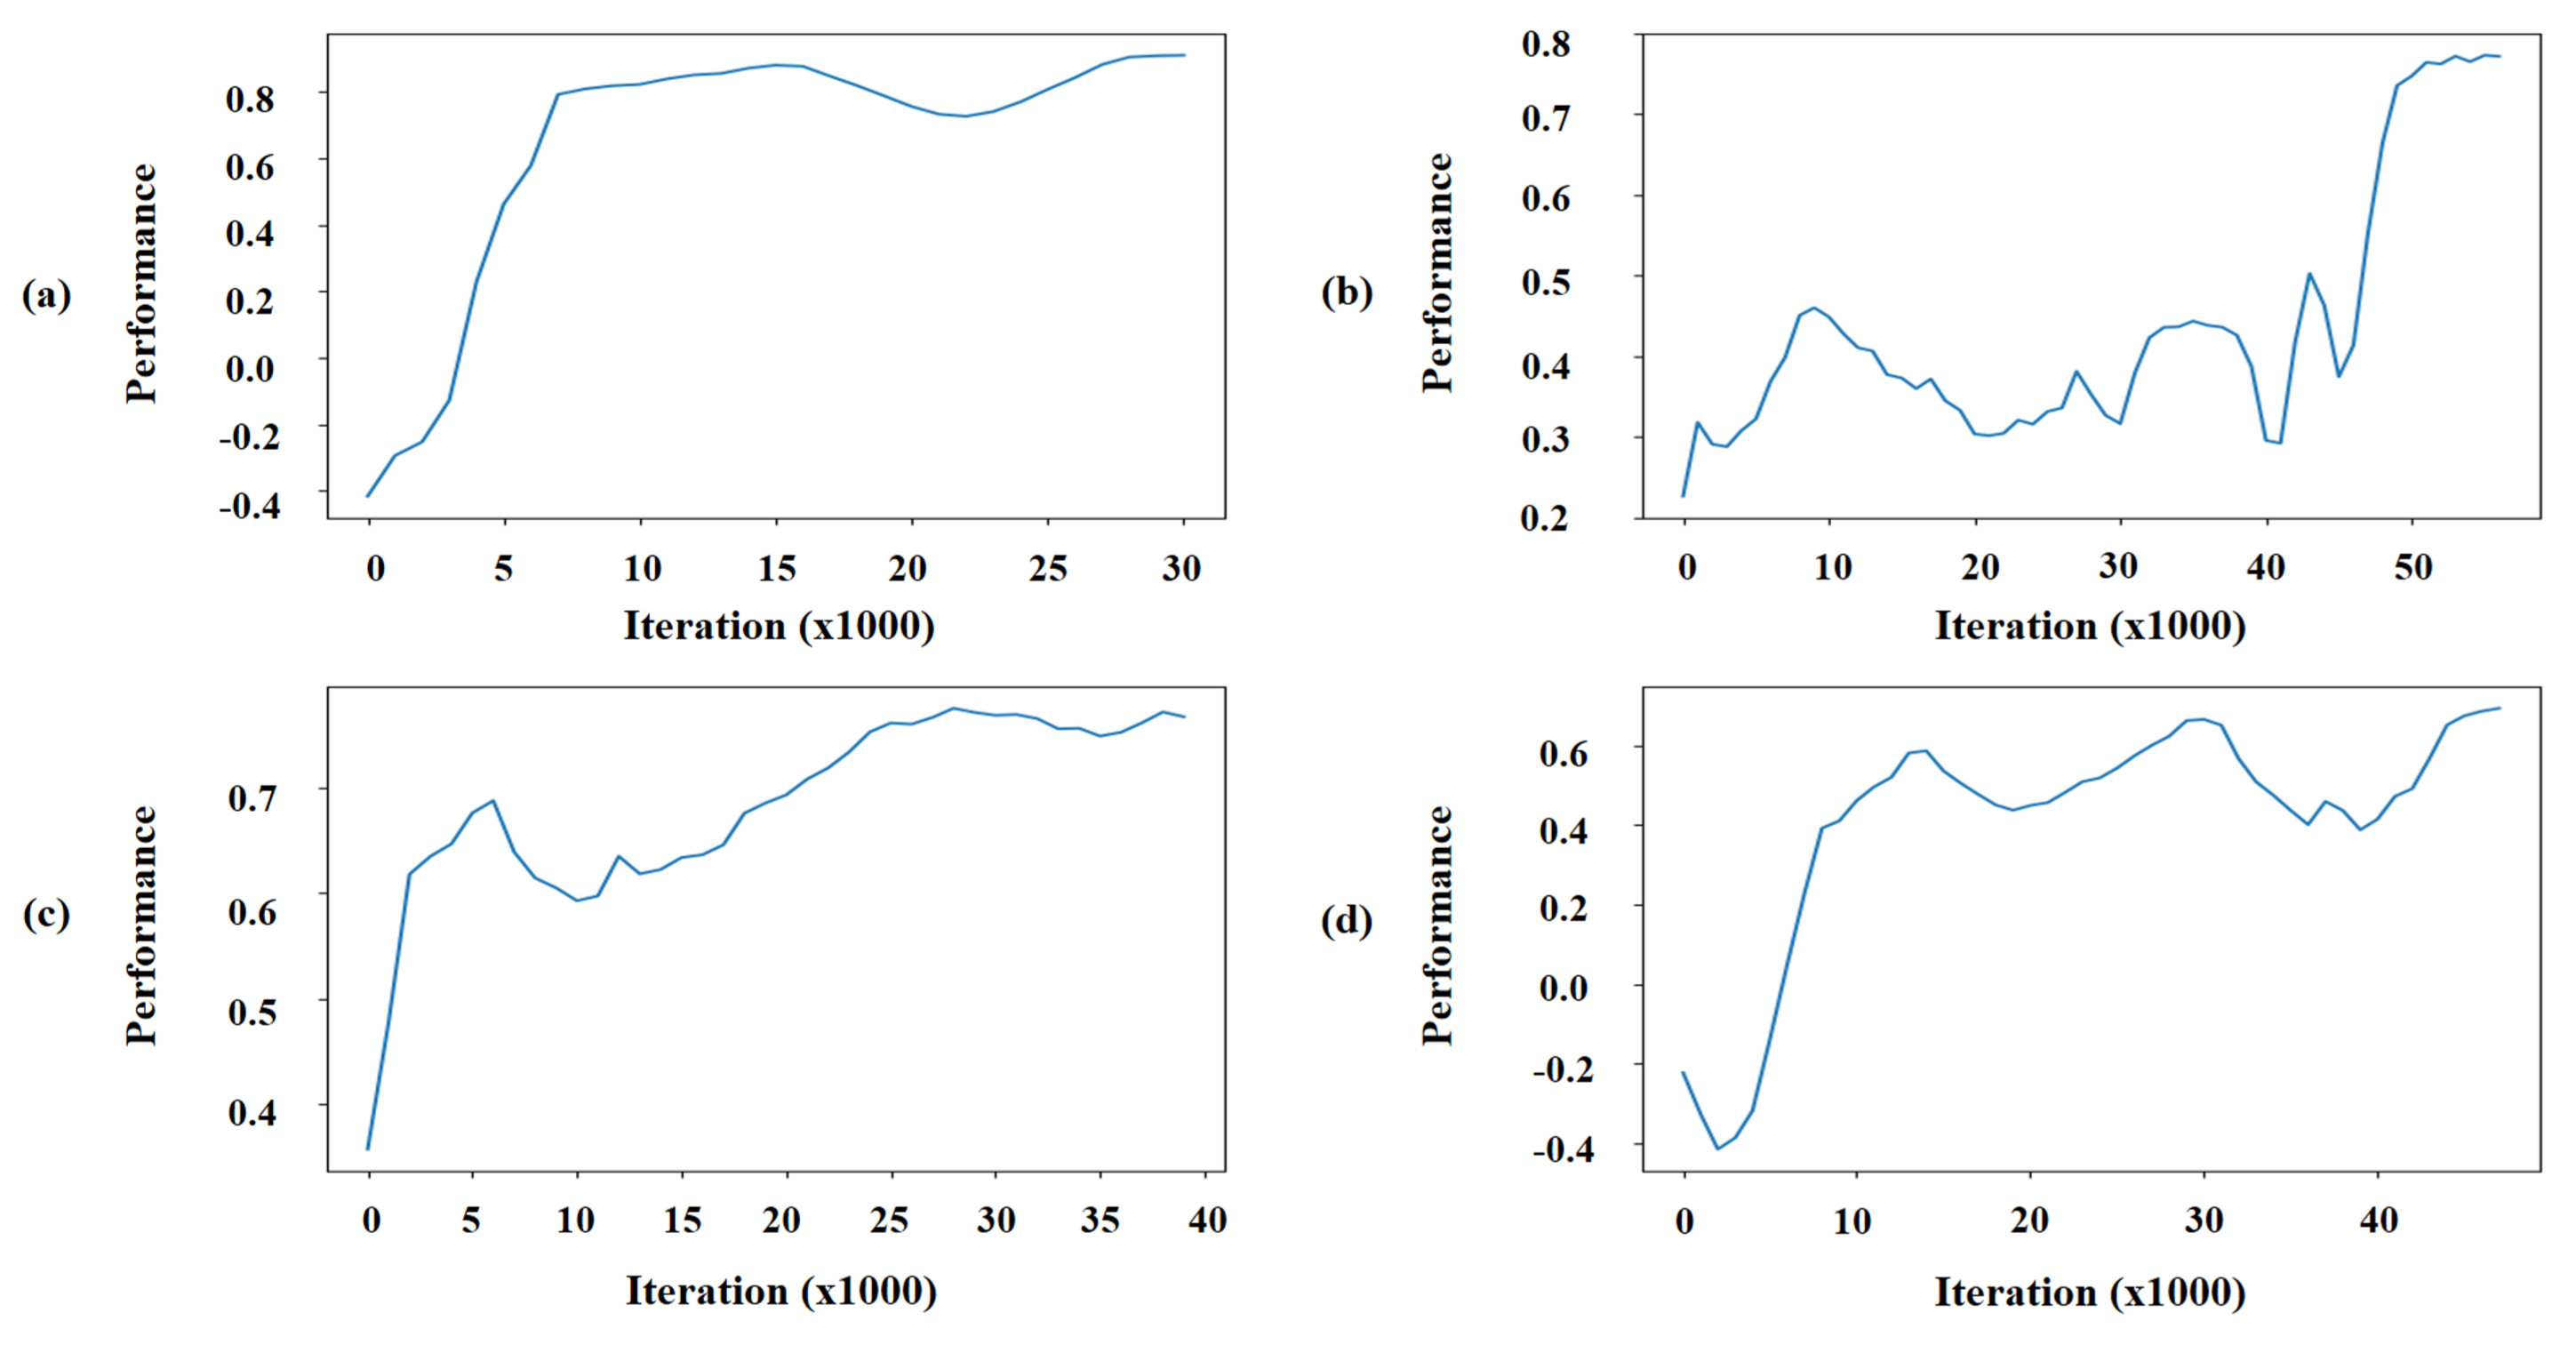
\includegraphics[width=1\linewidth]{images/aiPerformance.png}
  \caption{Performance Graphs for specifics scenarios, taken from \protect\cite{lee_crowd_2018}.}
  %Description{Performance Graphs for specifics scenarios}
  \label{fig:aiPerformance}
\end{figure}

\bibliographystyle{acmsiggraph}
\nocite{*}
\bibliography{literaturVerzeichnis}
\end{document}
